\chapter{Interpretable Graph Representations with NSPPK}
\label{ch:nsppk}


\section{Introduction}

Chapter~\ref{ch:theory} established the theoretical foundations of graph
representation learning and highlighted the complementary strengths of
predefined kernel methods and learned neural embeddings.
In particular, kernel-based representations offer deterministic feature
construction, transparent feature maps, and favourable behaviour in low-data
regimes, while neural approaches provide greater expressive flexibility at the
cost of increased training complexity and reduced transparency.

A key limitation identified in Chapter~\ref{ch:theory} concerns the treatment of
\emph{continuous node attributes} within scalable graph kernel frameworks.
Many classical kernels were originally designed for discretely labelled graphs
and rely on exact substructure matching. When applied to graphs with
real-valued features, these methods typically require discretisation or
hashing procedures that introduce artificial thresholds, reduce numerical
fidelity, and may distort similarity relationships. Although several extensions
incorporate continuous attributes through embeddings or propagation
mechanisms, they often sacrifice either scalability, robustness, or explicit
feature interpretability.

This chapter addresses this limitation by developing an explicit graph kernel
that integrates continuous node attributes directly into the feature
construction process while retaining the computational efficiency and
interpretability of classical substructure-based methods.

\paragraph{Chapter contribution.}
We introduce the \emph{Neighborhood Subgraph Pairwise Path Kernel} (NSPPK),
an explicit graph kernel that extends the
\emph{Neighborhood Subgraph Pairwise Distance Kernel}
(NSPDK)~\citep{costa2010fast}. While NSPDK compares fixed-radius neighbourhoods
around pairs of nodes, NSPPK enriches this representation to capture more
informative structural dependencies and to operate directly on real-valued node
features.

NSPPK advances prior work in three principal ways. First, it replaces
comparisons based solely on fixed-radius neighbourhoods with features derived
from unions of shortest-path neighbourhoods between node pairs, allowing the
representation to capture longer-range structural interactions. Second,
continuous node attributes are incorporated directly into the feature
construction without discretisation, preserving fine-grained information that
would otherwise be lost. Third, NSPPK produces explicit and sparse graph-level
embeddings, enabling kernel evaluation through efficient dot-product
computation. Under fixed parameters, feature extraction scales near-linearly
with graph size and the overall procedure is naturally parallelisable.

The empirical sections test whether this explicit construction can remain
accurate, scalable, and interpretable on attributed graph benchmarks. The
analysis focuses on predictive performance, runtime behaviour, feature
inspection, robustness to perturbations, and larger citation-network case
studies.

The remainder of this chapter is organised as follows.
Section~\ref{sec:relatedwork} reviews the graph-kernel literature most closely
related to NSPPK.
Section~\ref{sec:notation} introduces the NSPPK-specific notation and core
objects.
Section~\ref{sec:method} presents the feature construction and hashing scheme.
Section~\ref{sec:complexity} analyses computational complexity.
Section~\ref{sec:Diagonal} reports a controlled robustness analysis.
Section~\ref{sec:experiments} reports empirical results.
Section~\ref{sec:nsppk:discussion-limitations} discusses limitations.
Section~\ref{sec:Conclusion} concludes the chapter.

\section{Related Work}
\label{sec:relatedwork}

Chapter~\ref{ch:theory} situated graph kernels within the broader landscape of
graph representation learning, distinguishing explicit, predefined
representations from learned neural embeddings, and highlighted the particular
difficulty of handling continuous node attributes in scalable and interpretable
kernel frameworks. In this chapter, we therefore focus on the graph-kernel
literature most directly related to NSPPK.

Many graph kernels are formulated within the \emph{R-convolution} framework

\citep{haussler1999}, which defines similarities between structured objects by
decomposing them into collections of substructures and aggregating comparisons
over these parts. Within this family, the most direct predecessor of NSPPK is
the Neighborhood Subgraph Pairwise Distance Kernel (NSPDK)
\citep{costa2010fast}, which compares pairs of rooted neighbourhoods at fixed
graph distances. NSPDK is scalable and interpretable, but it was originally
designed for discrete labels and represents interactions between anchors only
through local neighbourhoods and their pairwise distance.

Several graph kernels have been proposed to extend this paradigm to continuous
node attributes. Propagation kernels \citep{neumann2016propagation} achieve
near-linear runtime by diffusing and hashing node attributes, but rely on
discretisation and may lose fine-grained numerical information. GraphHopper
\citep{feragen2013scalable} extends shortest-path kernels to attributed graphs
through node kernels evaluated along shortest paths, but remains
computationally more expensive and does not yield sparse explicit graph-level
feature maps. Wasserstein Weisfeiler--Lehman
\citep{togninalli2019wasserstein} replaces exact substructure matching with
optimal transport between distributions of refined node embeddings, increasing
flexibility at the cost of dense representations and higher computational
overhead.

More recent approaches such as MMD-GK \citep{mmdgk_iclr2024}, SWWL
\citep{carpintero2024swwl}, and DSP \citep{ye2025dsp} further shift away from
explicit combinatorial substructures by representing graphs as distributions of
node-, subgraph-, or path-level embeddings. These methods avoid strict discrete
matching, but typically rely on dense similarity computations, distribution
matching, or learned substructure representations, which can reduce
interpretability and increase memory and runtime requirements.

As discussed in Chapter~\ref{ch:theory}, graph neural networks provide an
alternative route for handling continuous attributes, since they learn
representations directly from graph structure and features. However, they are
training-based, task-dependent, and generally less interpretable than explicit
kernel features. In this chapter, they therefore serve primarily as empirical
baselines rather than direct methodological predecessors.

In contrast, NSPPK remains firmly within the explicit substructure-kernel para
digm. It extends NSPDK by enriching anchor-pair comparisons with unions of
shortest paths and by integrating continuous node attributes directly into the
explicit feature construction, without discretisation. In doing so, it aims to
occupy the methodological space identified in Chapter~\ref{ch:theory}: an
interpretable, deterministic, and scalable graph representation that retains
the advantages of explicit kernels while better supporting attributed graphs.





\section{Method}
\label{sec:method}

  A common strategy for defining kernels over structured objects is to decompose
them into collections of \emph{substructures} and compare these using a base
kernel. Kernels of this form fall under the \emph{R-convolution}
framework~\citep{haussler1999}, which subsumes many classical graph kernels.

A representative example is the Neighborhood Subgraph Pairwise Distance Kernel
(NSPDK)~\citep{costa2010fast}, which compares pairs of rooted neighbourhoods
whose centers lie at a prescribed graph distance. NSPDK yields explicit sparse
feature maps through permutation-invariant hashing, making feature extraction
efficient and kernel evaluation reducible to a sparse dot product.

Despite these strengths, NSPDK has two important limitations in the present
setting. First, it relies on exact matching of discrete node labels and thus
does not directly support real-valued node attributes. Second, its structural
features are defined only through pairs of fixed-radius neighbourhoods and their
distance. In graphs with high-degree nodes or multiple alternative routes
between anchors, this representation can become overly instance-specific:
similar neighbourhoods may fail to recur across graphs, feature overlap becomes
sparse, and the Gram matrix may become diagonally dominant, reducing
statistical coupling between training instances.

To address these limitations, we introduce the
\emph{Neighborhood Subgraph Pairwise Path Kernel} (NSPPK). NSPPK retains the
explicit and hash-based construction of NSPDK, but augments it in two
directions. Structurally, it enriches anchor-pair features with a connector
subgraph defined by the union of all shortest paths between the anchors,
thereby encoding more than distance alone. Attribute-wise, it integrates
continuous node attributes directly into the explicit feature construction,
avoiding discretisation while preserving fine-grained information in a
deterministic and interpretable representation.

\subsection{Core objects and notation}
\label{sec:notation}

We adopt the graph-theoretic notation introduced in
Chapter~\ref{ch:theory}, including shortest-path distance, induced subgraphs,
and $r$-hop neighbourhoods. Here we define only the additional objects that are
specific to NSPPK.

\textbf{Anchor pairs.}
We consider unordered anchor pairs $\{u,v\}\subseteq V$ such that $u$ and $v$
belong to the same connected component and have finite shortest-path distance
$d(u,v)\leq D$. Disconnected pairs are ignored.


\textbf{Union of shortest paths.}
For two vertices $u,v\in V$ with finite shortest-path distance, let $U(u,v)$
denote the subgraph induced by the union of all shortest $u$--$v$ paths.
Thus, $U(u,v)$ contains exactly the vertices and edges that belong to at least
one shortest path between $u$ and $v$.

\textbf{Connector subgraph.}
For a vertex set $S\subseteq V$, let $N_{r'}(S)$ denote the induced subgraph on
all vertices within shortest-path distance at most $r'$ from $S$, namely
\[
N_{r'}(S)
=
G\!\left[\{x\in V : \min_{s\in S} d(x,s)\le r'\}\right].
\]
For a connector radius $r'\ge 0$, we define the connector subgraph
\[
C_{r'}(u,v)
=
N_{r'}\!\big(U(u,v)\big).
\]
Thus, $C_0(u,v)=U(u,v)$, while $r'>0$ thickens the connector by including all
vertices within $r'$ hops of the path-union subgraph.

\textbf{NSPPK feature primitives.}
An NSPPK feature is defined by a pair of anchor neighbourhoods
\[
\bigl(N_{r_u}(u),\,N_{r_v}(v)\bigr),
\]
whose centers are at shortest-path distance $d(u,v)$, optionally augmented with
a connector subgraph $C_{r'}(u,v)$. Each feature is therefore parameterised by
a tuple $(r_u,r_v,d,r')$ and is invariant to permutations of vertices within
the constituent subgraphs.

\subsection{Augmented structural features}

NSPPK extends the feature family of NSPDK by augmenting pairs of rooted
neighbourhoods with an explicit connector subgraph
$C_{r'}(u,v)=N_{r'}(U(u,v))$. Whereas NSPDK represents the interaction between
two anchors only through the distance between them, NSPPK additionally encodes
the structure of the region connecting them.This idea is illustrated in Figure~\ref{fig:example}, which shows how NSPPK
augments two anchor neighbourhoods with a connector subgraph derived from the
union of shortest paths between them.This design is motivated by the observation that, although the number of
distinct shortest paths between two nodes may grow rapidly in graphs with many
cycles or alternative routes, their \emph{union} is uniquely defined as a
single subgraph. This yields a deterministic connector representation that
avoids combinatorial explosion while still capturing the multiplicity and
arrangement of shortest-path alternatives. As shown in Figure~\ref{fig:example}, two anchor pairs may have the same local
neighbourhood radii and the same anchor distance, yet differ in the internal
structure of the connector.

The NSPPK feature family is obtained by enumerating all parameter
configurations
\[
r_u,r_v \in \{0,\ldots,R\},\qquad
d \in \{0,\ldots,D\},\qquad
r' \in \{0,\ldots,R'\}\cup\{\varnothing\},
\]
where $R$, $D$, and $R'$ are small positive integers chosen for tractability.
The special value $r'=\varnothing$ denotes the case in which no connector is
included, recovering a neighbourhood-pair feature analogous to NSPDK.
Figure~\ref{fig:nspdk-vs-nsppk-example} provides a concrete comparison between
the two constructions, showing that the connector allows NSPPK to distinguish
cases that collapse to the same NSPDK feature.
\begin{figure}[t]
  \centering
  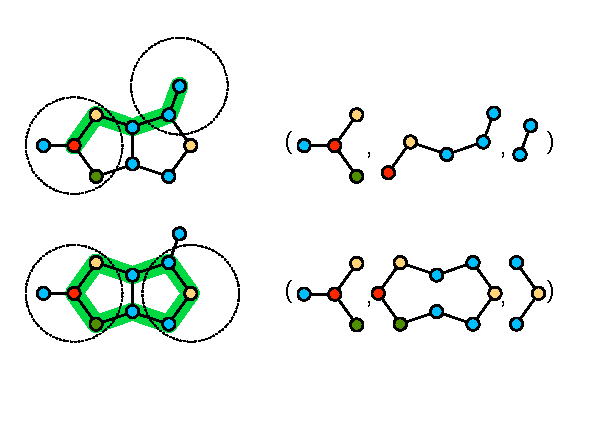
\includegraphics[width=0.65\textwidth]{images/nsppk_features.pdf}
    \caption{Example NSPPK structural features. Top: two radius-1 neighbourhoods
    centred at an anchor pair whose vertices are at shortest-path distance 4,
    together with their union-of-shortest-paths connector for $r'=0$, corresponding
    to a single shortest path. Bottom: an analogous anchor-pair configuration in
    which the two anchors are again at distance 4, but the connector contains two
    distinct shortest paths of length 4.}
  \label{fig:example}
\end{figure}

\subsection{From subgraphs to explicit features}

Rather than defining similarity directly between graphs, NSPPK first enumerates
a family of local subgraph patterns. Each pattern is determined by a pair of
anchor neighbourhoods at given radii, together with an optional connector
subgraph derived from the union of shortest paths between the anchors. Every
such configuration is then mapped, through permutation-invariant hashing, to a
feature identifier. A graph is finally represented by a sparse histogram
counting how often each feature occurs.

Formally, let $\theta=(R,D,R')$ denote the maximal radii and distances used in
feature extraction. For a graph $G$, let $f_G^\theta$ denote the vector of NSPPK
feature counts. The kernel between two graphs $G$ and $G'$ is defined as
\[
k_\theta(G,G')
=
{f_G^\theta}^{\top} f_{G'}^\theta.
\]

Because NSPPK features are extracted from unordered anchor pairs, the
graph-level feature vector decomposes as
\[
f_G^\theta
=
\sum_{\substack{\{u,v\}\subseteq V\\u\neq v,\ d(u,v)\le D}}
f_{G,u,v}^\theta,
\]
where $f_{G,u,v}^\theta$ denotes the contribution associated with anchor pair
$\{u,v\}$.

\subsection{Feature hashing pipeline}

To obtain an explicit sparse representation, each structural pattern is mapped
to a hash bucket. Let $b$ denote the number of hash bits. The hash codomain therefore has size
\[
M = 2^b.
\]
Using hashed identifiers allows constant-time indexing into the feature vector
and avoids explicit subgraph isomorphism checks.

A practical advantage of NSPPK is that hashes can be computed
\emph{incrementally} with respect to neighbourhood radius and shortest-path
distance, and cached for reuse. In particular, rooted neighbourhood hashes are
computed once per node and reused when forming neighbourhood-pair and connector
features, avoiding repeated recomputation over anchor pairs.

\textbf{Base hash functions.}
We use SHA-256 as a deterministic hashing function. For any object $x$, let
$\mathrm{sha256}(x)$ denote the integer obtained by applying SHA-256 to a
canonical serialisation of $x$. We define the corresponding $b$-bit base hash as
\[
H_b(x)=\mathrm{sha256}(x)\bmod 2^b.
\]
From $H_b$, we derive two composite operators. First, $H^q(I)$ denotes the
\emph{sequence hash} of an ordered tuple $I=(x_1,\dots,x_k)$, and therefore
preserves the order of its elements. Second, $H^t(S)$ denotes the
\emph{multiset hash} of a multiset $S$; it is computed after lexicographic
sorting and is therefore invariant to permutations of the elements. These two
operators allow NSPPK to distinguish between ordered structural compositions
when order is meaningful, while remaining permutation-invariant for unordered
collections such as neighbourhood shells.

\textbf{Node hash.}
For each node $v$, define the incident-neighbour multiset hash
\[
N_h(v)
=
H^t\!\left(
\{\!\!\{
H^q\big([H_b(\ell(u)), H_b(\ell(e_{v,u}))]\big)
:
u \in N(v)
\}\!\!\}
\right),
\]
and define the rooted node hash as
\[
N_H(v)
=
H^q\big([H_b(\ell(v)), N_h(v)]\big).
\]
When edge labels are unavailable, $\ell(e_{v,u})$ is replaced by a fixed dummy
label.

\textbf{Rooted neighbourhood hash.}
For a node $v$ and shell index $j\ge 0$, let
\[
D_j^v=\{\,u\in V : d(v,u)=j\,\}
\]
be the set of nodes at exact distance $j$ from $v$. Define the shell hash
\[
B_j^v
=
H^t\bigl(\{\!\!\{\,N_H(u) : u\in D_j^v\,\}\!\!\}\bigr),
\]
and then the rooted neighbourhood hash of radius $r$ by
\[
G_H^r(v)
=
H^q([B_0^v,B_1^v,\dots,B_r^v]).
\]
These hashes are computed incrementally in $r$ and cached for each node.

\textbf{Neighbourhood-pair hash.}
For an anchor pair $(u,v)$ at distance $d=d(u,v)$, define
\[
P_H^{r_u,r_v,d}(u,v)
=
H^q\!\left(
\left[
H_b(d),
H^t\!\left(
\left\{\!\!\left\{
H^q([H_b(r_u),G_H^{r_u}(u)]),
H^q([H_b(r_v),G_H^{r_v}(v)])
\right\}\!\!\right\}
\right)
\right]
\right).
\]

\textbf{Connector hash.}
To encode the connector deterministically, we organise its nodes into distance
shells from one anchor node $u$ along the path-union subgraph. Let $U(u,v)$ be
the union of all shortest $u\leftrightarrow v$ paths. We use the notation
$\overline{B}_{j,r'}(u,v)$ to denote a \emph{connector shell hash}, analogous to
the neighbourhood shell hash $B_j^v$ but restricted to nodes lying in the
connector subgraph and constructed from rooted neighbourhood hashes
$G_H^{r'}(\cdot)$ rather than node hashes $N_H(\cdot)$. For each shell index
$j\in\{0,\dots,d(u,v)\}$, define
\[
\overline{B}_{j,r'}(u,v)
=
H^t\bigl(
\{\!\!\{\,G_H^{r'}(w) : w\in D_j^{\,u}\cap V(U(u,v))\,\}\!\!\}
\bigr),
\]
where $V(U(u,v))$ is the vertex set of the path-union subgraph. The connector
hash is then
\[
U_H^{r',d}(u,v)
=
H^q\!\left(
[\overline{B}_{0,r'}(u,v),\dots,\overline{B}_{d,r'}(u,v)]
\right).
\]

\textbf{Final structural feature vector.}
The structural NSPPK vector is obtained by accumulating the hash values of all
neighbourhood-pair and connector features extracted from the graph. The
practical effect of including the connector is illustrated in
Figure~\ref{fig:nspdk-vs-nsppk-example}. Two graphs that are indistinguishable
to NSPDK because they share the same anchor neighbourhoods and anchor distance
are separated by NSPPK once the connector structure is incorporated.

\begin{figure*}[h]
  \centering
  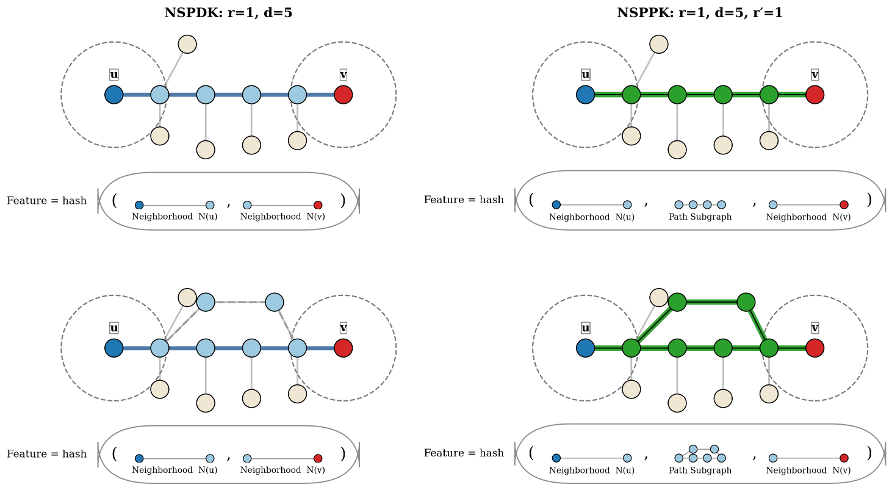
\includegraphics[width=0.95\textwidth]{images/nspdk_vs_nsppk_networkx.png}
  \caption{\textbf{NSPDK vs.\ NSPPK on anchors $u,v$ with $r=1$ and $d=5$.}
  \emph{Left:} NSPDK features for the case with a single shortest path (top) and
  two equal-length shortest paths (bottom). Because NSPDK uses only
  $(N_r(u),d(u,v),N_r(v))$, both cases produce the same feature.
  \emph{Right:} NSPPK includes the connector
  $C_{r'}(u,v)=N_{r'}(U(u,v))$ (shown in green). The connector is a simple path
  in the top graph but a two-path union in the bottom graph, so NSPPK induces
  different features.}
  \label{fig:nspdk-vs-nsppk-example}
\end{figure*}

\subsection{Node attribute integration}
\label{subsec:attribute_integration}

We now extend the structural feature map to graphs with continuous node
attributes. Let
\[
X\in\mathbb{R}^{n\times p}
\]
denote the node-attribute matrix, where each row corresponds to a node and each
column to one of the $p$ attributes. Let
\[
F\in\mathbb{R}^{n\times M}
\]
denote the binary node--feature incidence matrix, where $M=2^b$ is the number of hash buckets and $F_{ij}=1$ if node $i$ contributes to structural feature
$j$. We then define the attribute-augmented representation by
\[
x = \mathrm{vec}(X^\top F)\in\mathbb{R}^{pM}.
\]

In this construction, each structural bucket stores the aggregated continuous
attributes of the nodes contributing to that feature. Thus, structural identity
and continuous attributes are combined within a single explicit feature map.
Node weights can be incorporated by replacing $X$ with $\mathrm{diag}(w)X$,
where $w\in\mathbb{R}^n$ is a vector of node weights. The same mechanism
extends naturally to edge attributes. NSPPK feature extraction remains entirely
deterministic and training-free; supervised learning is introduced only by the
downstream classifier applied to the resulting explicit graph representation.

\subsection{Expressivity Relative to NSPDK and Local Aggregation}
\label{sec:isomorphism}

Distinguishing non-isomorphic graphs is a key requirement for expressive graph
kernels. Two graphs $G=(V_G,E_G)$ and $H=(V_H,E_H)$ are \emph{isomorphic},
denoted $G\cong H$, if there exists a bijection $\pi:V_G\to V_H$ that
preserves adjacency. A valid graph kernel should at least be
\emph{isomorphism-invariant}, meaning that its value does not depend on vertex
ordering. More strongly, one seeks \emph{isomorphism-discrimination}, namely the
ability to assign different similarities to non-isomorphic graphs whenever
their structural differences are visible to the feature map.

The expressive power of many classical graph kernels and message-passing graph
neural networks is closely tied to the
\emph{1-dimensional Weisfeiler--Lehman (1-WL)} test
\citep{shervashidze2011weisfeiler,morris2019weisfeiler}. In particular,
graphs that are indistinguishable by 1-WL cannot be separated by WL-based
kernels, and standard message-passing GNNs are likewise bounded by 1-WL in
distinguishing power \citep{xu2019powerful}. Although higher-order WL variants
can increase expressivity, they generally do so at substantially higher
computational cost.

NSPPK complements local aggregation by encoding not only rooted neighbourhoods
around anchor nodes, but also the connector structure between them. Its
features have the form
\[
\psi\bigl(N_{r_u}(u),\,C_{r'}(u,v),\,N_{r_v}(v)\bigr),
\]
where $\psi(\cdot)$ denotes the NSPPK feature identifier associated with the
anchor neighbourhoods and connector, and
$C_{r'}(u,v)=N_{r'}(U(u,v))$ is derived from the union of all shortest paths
between the anchors. Consequently, two graphs may share identical local anchor
neighbourhoods and the same anchor distance, yet still be separated by NSPPK iif the connector encodings produced by NSPPK differ.

Figure~\ref{fig:isomorphism} illustrates graph pairs that standard local
aggregation schemes fail to distinguish reliably from neighbourhood information
alone. NSPPK can separate such pairs by explicitly encoding the shortest-path
connectivity pattern between anchors rather than relying only on local rooted
structure.
% ---- Figure 1 ----
\begin{figure}[H]
\centering
\begin{adjustbox}{max width=\linewidth}
\begin{tikzpicture}[x=1cm,y=1cm, line cap=round, line join=round,
                    every node/.style={outer sep=0pt}]

  \tikzset{
    panel/.style={rounded corners=2mm, draw=black!20, fill=black!2, line width=0.4pt},
    edge/.style={line width=0.95pt, draw=black!70},
    vblue/.style={circle, draw=blue!55!black, fill=blue!40, minimum size=6.2pt, inner sep=0pt},
    vgreen/.style={circle, draw=teal!55!black, fill=teal!40, minimum size=6.2pt, inner sep=0pt},
    vred/.style={circle, draw=red!55!black, fill=red!40, minimum size=6.2pt, inner sep=0pt},
    vyellow/.style={circle, draw=orange!55!black, fill=orange!40, minimum size=6.2pt, inner sep=0pt}
  }

  \node[panel, minimum width=7.6cm, minimum height=3.6cm, anchor=center] (A) at (0,0) {};
  \node[panel, minimum width=7.6cm, minimum height=3.6cm, anchor=center] (B) at (8.8,0) {};
  \node[anchor=west] at ([xshift=-3.6cm,yshift=1.55cm]A.center) {\small\textbf{(a)}};
  \node[anchor=west] at ([xshift=-3.6cm,yshift=1.55cm]B.center) {\small\textbf{(b)}};

  \path[use as bounding box]
    ([xshift=-1mm,yshift=-1mm]A.south west)
      rectangle
    ([xshift=+1mm,yshift=+1mm]B.north east);

  % Panel (a)
  \begin{scope}
    \clip[rounded corners=2mm] (A.south west) rectangle (A.north east);

    \def\R{1.15}
    \foreach \i in {0,...,5} \coordinate (h\i) at ($([xshift=-2.2cm]A.center) + (\i*60:\R)$);
    \foreach \i/\j in {0/1,1/2,2/3,3/4,4/5,5/0} \draw[edge] (h\i)--(h\j);
    \foreach \i in {0,...,5} \node[vblue] at (h\i) {};

    \coordinate (S) at ($([xshift=+2.1cm]A.center)$);
    \coordinate (u1) at ($(S)+(-1.15,  0.55)$);
    \coordinate (u2) at ($(S)+(-0.45,  0.55)$);
    \coordinate (u3) at ($(S)+(-0.80, -0.40)$);
    \coordinate (v1) at ($(S)+( 0.45, -0.55)$);
    \coordinate (v2) at ($(S)+( 1.15, -0.55)$);
    \coordinate (v3) at ($(S)+( 0.80,  0.40)$);
    \foreach \a/\b in {u1/u2,u2/u3,u3/u1,v1/v2,v2/v3,v3/v1} \draw[edge] (\a)--(\b);
    \foreach \p in {u1,u2,u3,v1,v2,v3} \node[vgreen] at (\p) {};
  \end{scope}

  % Panel (b)
  \begin{scope}
    \clip[rounded corners=2mm] (B.south west) rectangle (B.north east);
    \coordinate (c)  at ($([xshift=-2.2cm]B.center)+(0,0)$);
    \coordinate (l1) at ($([xshift=-2.2cm]B.center)+(-0.9, 0.7)$);
    \coordinate (l2) at ($([xshift=-2.2cm]B.center)+(-1.2,-0.6)$);
    \coordinate (r1) at ($([xshift=-2.2cm]B.center)+( 0.9, 0.7)$);
    \coordinate (r2) at ($([xshift=-2.2cm]B.center)+( 1.2,-0.6)$);
    \foreach \a/\b in {l1/c,c/l2,l2/l1,r1/c,c/r2,r2/r1} \draw[edge] (\a)--(\b);
    \foreach \p in {l1,l2,c,r1,r2} \node[vred] at (\p) {};

    \coordinate (g00) at ($([xshift=+2.0cm]B.center)+(-1.2, 0.6)$);
    \coordinate (g01) at ($([xshift=+2.0cm]B.center)+(-1.2,-0.6)$);
    \coordinate (g10) at ($([xshift=+2.0cm]B.center)+( 0.0, 0.6)$);
    \coordinate (g11) at ($([xshift=+2.0cm]B.center)+( 0.0,-0.6)$);
    \coordinate (g20) at ($([xshift=+2.0cm]B.center)+( 1.2, 0.6)$);
    \coordinate (g21) at ($([xshift=+2.0cm]B.center)+( 1.2,-0.6)$);
    \foreach \a/\b in {g00/g10,g10/g20,g01/g11,g11/g21} \draw[edge] (\a)--(\b);
    \foreach \a/\b in {g00/g01,g10/g11,g20/g21} \draw[edge] (\a)--(\b);
    \foreach \p in {g00,g01,g10,g11,g20,g21} \node[vyellow] at (\p) {};
  \end{scope}
\end{tikzpicture}
\end{adjustbox}
\caption{Illustrative graph pairs that local neighbourhood-based methods may fail
to distinguish, but which NSPPK can separate by encoding connector structure.
\textbf{(a)} \(C_6\) vs.\ \(K_3 \cup K_3\) (two disconnected triangles).
\textbf{(b)} Bow-tie vs.\ \(2\times3\) grid (“ladder”).}
\label{fig:isomorphism}
\end{figure}
\paragraph{NSPPK vs.\ NSPDK.}
This distinction is especially important relative to NSPDK.
NSPDK features depend only on pairs of rooted neighbourhoods and the distance
between their centres. Thus, if two graphs agree on these quantities up to a
fixed radius budget, NSPDK assigns them the same representation even when the
connector structure between the anchors differs. By contrast, NSPPK augments
anchor-pair features with the union-of-shortest-paths connector and can
therefore distinguish graphs that are locally identical around the anchors but
differ in how those anchors are linked.

As illustrated in Figure~\ref{fig:nsppk-vs-nspdk-hexagon}, this yields a
strict separation under fixed local radii. In particular, there exist
non-isomorphic graph pairs for which NSPDK produces identical features for the
chosen anchor radius, whereas NSPPK assigns distinct features by encoding the
connector structure.

\begin{proposition}[NSPPK separates configurations with distinct connector encodings]
\label{prop:nsppk_separates_nspdk}
Let $G$ and $H$ be two graphs containing anchor pairs $(u,v)$ and $(u',v')$,
respectively. Suppose that, for a fixed radius $r$, the rooted neighbourhoods
around the anchors agree,
\[
N_r(u)\cong N_r(u')
\qquad\text{and}\qquad
N_r(v)\cong N_r(v'),
\]
and that the anchor distances are equal,
\[
d(u,v)=d(u',v').
\]
Then NSPDK assigns the same feature to these two anchor configurations under
idealised isomorphism-aware hashing.

Suppose, however, that for some connector radius $r'\geq 0$, the connector
encodings produced by the NSPPK procedure for $C_{r'}(u,v)$ and
$C_{r'}(u',v')$ are distinct. Then the corresponding NSPPK anchor features are
also distinct, except in the event of a finite-bit hash collision.
\end{proposition}





\begin{proof}
NSPDK represents an anchor configuration using the rooted neighbourhoods around
the two anchors and the distance between them. Therefore, under the assumptions
\[
N_r(u)\cong N_r(u'),
\qquad
N_r(v)\cong N_r(v'),
\qquad
d(u,v)=d(u',v'),
\]
the two configurations receive the same NSPDK feature under idealised
isomorphism-aware hashing.

NSPPK additionally incorporates a connector encoding into the anchor-pair
feature. If the connector encodings produced for $C_{r'}(u,v)$ and
$C_{r'}(u',v')$ are distinct, then the corresponding pre-hash NSPPK feature
descriptions are distinct. Consequently, their finite-bit feature identifiers
are also distinct unless the two descriptions are mapped to the same hash
bucket through a collision.
\end{proof}

Figure~\ref{fig:nsppk-vs-nspdk-hexagon} illustrates a concrete instance. The
two graphs are locally indistinguishable around the chosen anchors and share
the same anchor distance, so NSPDK produces identical anchor-pair features.
NSPPK separates them because the union-of-shortest-paths connector has different
internal structure in the two cases.
% ---- Figure 2 ----
\begin{figure}[t]
  \centering
  \begin{adjustbox}{max width=0.95\linewidth}
  \begin{tikzpicture}[x=1cm,y=1cm, line cap=round, line join=round,
                      every node/.style={outer sep=0pt}]
    \tikzset{
      panel/.style={rounded corners=2mm, draw=black!20, fill=black!2, line width=0.4pt},
      edge/.style={line width=0.95pt, draw=black!70},
      vnode/.style={circle, draw=blue!55!black, fill=blue!40, minimum size=6.2pt, inner sep=0pt},
      vanchor/.style={circle, draw=blue!40, fill=blue!40, minimum size=7pt, inner sep=0pt}
    }

    \node[panel, minimum width=5.5cm, minimum height=3.6cm] (A) at (0,0) {};
    \node[panel, minimum width=5.5cm, minimum height=3.6cm] (B) at (6.6,0) {};
    \node[anchor=west] at ([xshift=-2.6cm,yshift=1.45cm]A.center) {\small\textbf{(a)}};
    \node[anchor=west] at ([xshift=-2.6cm,yshift=1.45cm]B.center) {\small\textbf{(b)}};

    \path[use as bounding box]
      ([xshift=-1mm,yshift=-1mm]A.south west)
        rectangle
      ([xshift=+1mm,yshift=+1mm]B.north east);

    % Panel (a)
    \begin{scope}
      \clip[rounded corners=2mm] (A.south west) rectangle (A.north east);
      \coordinate (C) at ([xshift=-0.1cm]A.center);
      \def\R{1.1}

      \foreach \i/\ang in {1/270,2/210,3/150,4/90,5/30,6/330}
        \coordinate (a\i) at ($(C)+(\ang:\R)$);

      \foreach \u/\v in {1/2,2/3,3/4,4/5,5/6,6/1} \draw[edge] (a\u)--(a\v);
      \foreach \u/\v in {2/3,3/5,5/6,6/2} \draw[edge] (a\u)--(a\v);

      \foreach \i in {2,3,5,6} \node[vnode] at (a\i) {};
      \node[vanchor] at (a1) {};
      \node[vanchor] at (a4) {};

      \foreach \i in {1,...,6}
        \node[font=\scriptsize, above=1pt] at (a\i) {\i};
    \end{scope}

    % Panel (b)
    \begin{scope}
      \clip[rounded corners=2mm] (B.south west) rectangle (B.north east);
      \coordinate (C2) at ([xshift=-0.1cm]B.center);
      \def\Rtwo{1.1}

      \foreach \i/\ang in {1/270,2/210,3/150,4/90,5/30,6/330}
        \coordinate (b\i) at ($(C2)+(\ang:\Rtwo)$);

      \foreach \u/\v in {1/2,2/3,3/4,4/5,5/6,6/1} \draw[edge] (b\u)--(b\v);
      \foreach \u/\v in {2/5,3/6} \draw[edge] (b\u)--(b\v);

      \foreach \i in {2,3,5,6} \node[vnode] at (b\i) {};
      \node[vanchor] at (b1) {};
      \node[vanchor] at (b4) {};

      \foreach \i in {1,...,6}
        \node[font=\scriptsize, above=1pt] at (b\i) {\i};
    \end{scope}
  \end{tikzpicture}
  \end{adjustbox}

\caption{\textbf{A concrete anchor configuration separated by NSPPK but not NSPDK.}
Both graphs share the same outer 6-cycle, and the chosen anchors, nodes $1$ and
$4$, have identical rooted neighbourhoods $N_r(1)$ and $N_r(4)$ for
$r\le R_0$ (here $R_0=1$), with the same anchor distance $d(1,4)$.
Therefore, NSPDK assigns the same feature to this anchor configuration.
\textbf{(a)} Inner square on nodes $\{2,3,5,6\}$.
\textbf{(b)} Inner cross via diagonals $(2,5)$ and $(3,6)$.
However, the connector $C_{r'}(1,4)$ differs: the union of shortest paths
$U(1,4)$ forms a cycle in (a) and two node-disjoint paths in (b). Hence, the two configurations produce distinct connector encodings under the
NSPPK procedure, except in the event of a finite-bit hash collision.}
\label{fig:nsppk-vs-nspdk-hexagon}
\end{figure}
\subsection{Complexity Analysis}
\label{sec:complexity}

The computational cost of NSPPK is dominated by truncated breadth-first
searches (BFS) used to extract local neighbourhoods and enumerate anchor pairs.
A detailed derivation of the computational and space complexity is provided in
Appendix~\ref{appendix:complexity}; here we summarize the main scaling behavior.

Let
\[
L_{\max}=\max(R,D,R').
\]

For a node $v\in V$ and radius $\ell\le L_{\max}$, define the radius-$\ell$
ball
\[
\mathcal{B}_\ell(v)=\{u\in V \mid d(u,v)\le \ell\},
\]
and let $E_\ell(v)$ denote the set of edges induced by this ball.
A BFS truncated at depth $\ell$ explores precisely this radius-$\ell$
neighbourhood, and therefore visits
\[
O\bigl(|\mathcal{B}_\ell(v)| + |E_\ell(v)|\bigr)
\]
vertices and edges.

Feature extraction consists of two main BFS-based phases.
First, in the \emph{neighbourhood hashing} phase, for each $v\in V$ a single BFS
to depth $R$ is used to compute all rooted neighbourhood hashes $G_H^r(v)$ for
$r\le R$, which are then cached and reused.
Second, in the \emph{pairwise enumeration} phase, for each $v\in V$ a BFS to
depth $D$ enumerates all anchor nodes $u$ such that $d(v,u)\le D$ and combines
their precomputed hashes, together with connector hashes when these are enabled.

The total structural feature-extraction cost is therefore
\[
O\!\left(
\sum_{v\in V}\bigl(|\mathcal{B}_R(v)|+|E_R(v)|\bigr)
+
\sum_{v\in V}\bigl(|\mathcal{B}_D(v)|+|E_D(v)|\bigr)
+
C_{\mathrm{conn}}
\right),
\]
where $C_{\mathrm{conn}}$ denotes the additional cost of constructing connector
hashes for the enumerated anchor pairs.

Under fixed radii $(R,D,R')$ and bounded effective degree
\[
K_{\mathrm{eff}}=\min(K,\tau),
\]
this yields the simplified bound
\[
O\bigl(|V|K_{\mathrm{eff}}^{L_{\max}}\bigr),
\]
up to constants depending on connector construction and hashing, where
$K=\max_{v\in V}\deg(v)$ is the maximum degree and $\tau$ is an optional degree
cutoff used to control feature explosion in high-degree graphs.

Hence, in the practically relevant regime of small radii and bounded effective
degree, NSPPK scales near-linearly with the number of nodes. A quadratic
$|V|^2$ anchor-enumeration regime can arise in dense or high-degree graphs where
truncated BFS neighbourhoods approach the full graph.

Incorporating $p$-dimensional continuous node attributes introduces a linear
factor in the attribute dimension, since each extracted structural feature
aggregates attribute vectors only from the nodes participating in that feature.
The overall cost therefore becomes
\[
O\bigl(p\,|V|K_{\mathrm{eff}}^{L_{\max}}\bigr)
\]
under the same bounded-degree assumptions.

\paragraph{Kernel evaluation.}
After feature extraction, each graph $G$ is represented by the sparse feature
count vector $f_G^\theta$, and kernel evaluation reduces to the sparse dot product
\[
k_\theta(G,G') = {f_G^\theta}^{\top} f_{G'}^\theta,
\]
with cost
\[
O\!\bigl(\mathrm{nnz}(f_G^\theta)+\mathrm{nnz}(f_{G'}^\theta)\bigr),
\]
where $\mathrm{nnz}(\cdot)$ denotes the number of nonzero entries.

In practice, this step is highly efficient and depends on the number of active
features rather than on the ambient dimensionality of the hash space. NSPPK
therefore combines explicit sparse representations with efficient feature
extraction. Its cost is governed by truncated local exploration, admits a
near-linear regime under fixed radii and bounded effective degree, and remains
practical because kernel evaluation itself reduces to sparse linear algebra.

\subsection{Balancing Feature Size and Hash Collisions}

The expressivity analysis in the previous section characterises the underlying
NSPPK feature family; in practice, these features are instantiated via finite-bit
hashing, which introduces collisions and motivates an empirical study of the
accuracy--collision trade-off. The number of hash bits controls the dimensionality
of the hashed feature codomain: fewer bits increase collision probability,
introducing noise and potentially reducing predictive accuracy, while larger bit
sizes (e.g., $b \ge 20$) yield very large feature spaces with higher memory
demands. Although sparse representations alleviate storage costs, excessively
large codomains may still become impractical for downstream learning models.

To examine this trade-off empirically, we trained a random forest classifier on
1{,}300 molecular graphs from PubChem AID~463230 (pPAFAH inhibition assay),
excluding node attributes. As shown in
Figure~\ref{fig:bits_tradeoff}\subref{fig:nbit-a}, predictive performance
degrades only gradually as the bit size decreases and remains stable even at
approximately 14 bits (about 16k features), despite collision rates exceeding
10\%. This indicates that collisions among infrequent features are largely
tolerated, enabling compact yet effective representations.

As a separate scalability check, we evaluate the computational impact of the
number of hash bits on the large QM9 dataset~\citep{ramakrishnan2014quantum},
which contains roughly 129{,}000 molecular graphs with 16 continuous node
attributes. This experiment is not intended to explain the collision--accuracy
trade-off in Figure~\ref{fig:bits_tradeoff}\subref{fig:nbit-a}; rather, it
measures how the dimensionality of the hashed feature space affects
vectorisation time on a substantially larger attributed dataset. As shown in
Figure~\ref{fig:bits_tradeoff}\subref{fig:nsppk_qm9-a}, vectorisation time
generally increases with the number of hash bits, while remaining practical for
moderate settings. Additional discussion of the QM9 vectorisation-time
experiment is provided in Appendix~\ref{appendix:qm9}.

\begin{figure}[t]
  \centering

  \begin{subfigure}[t]{0.45\linewidth}
    \centering
    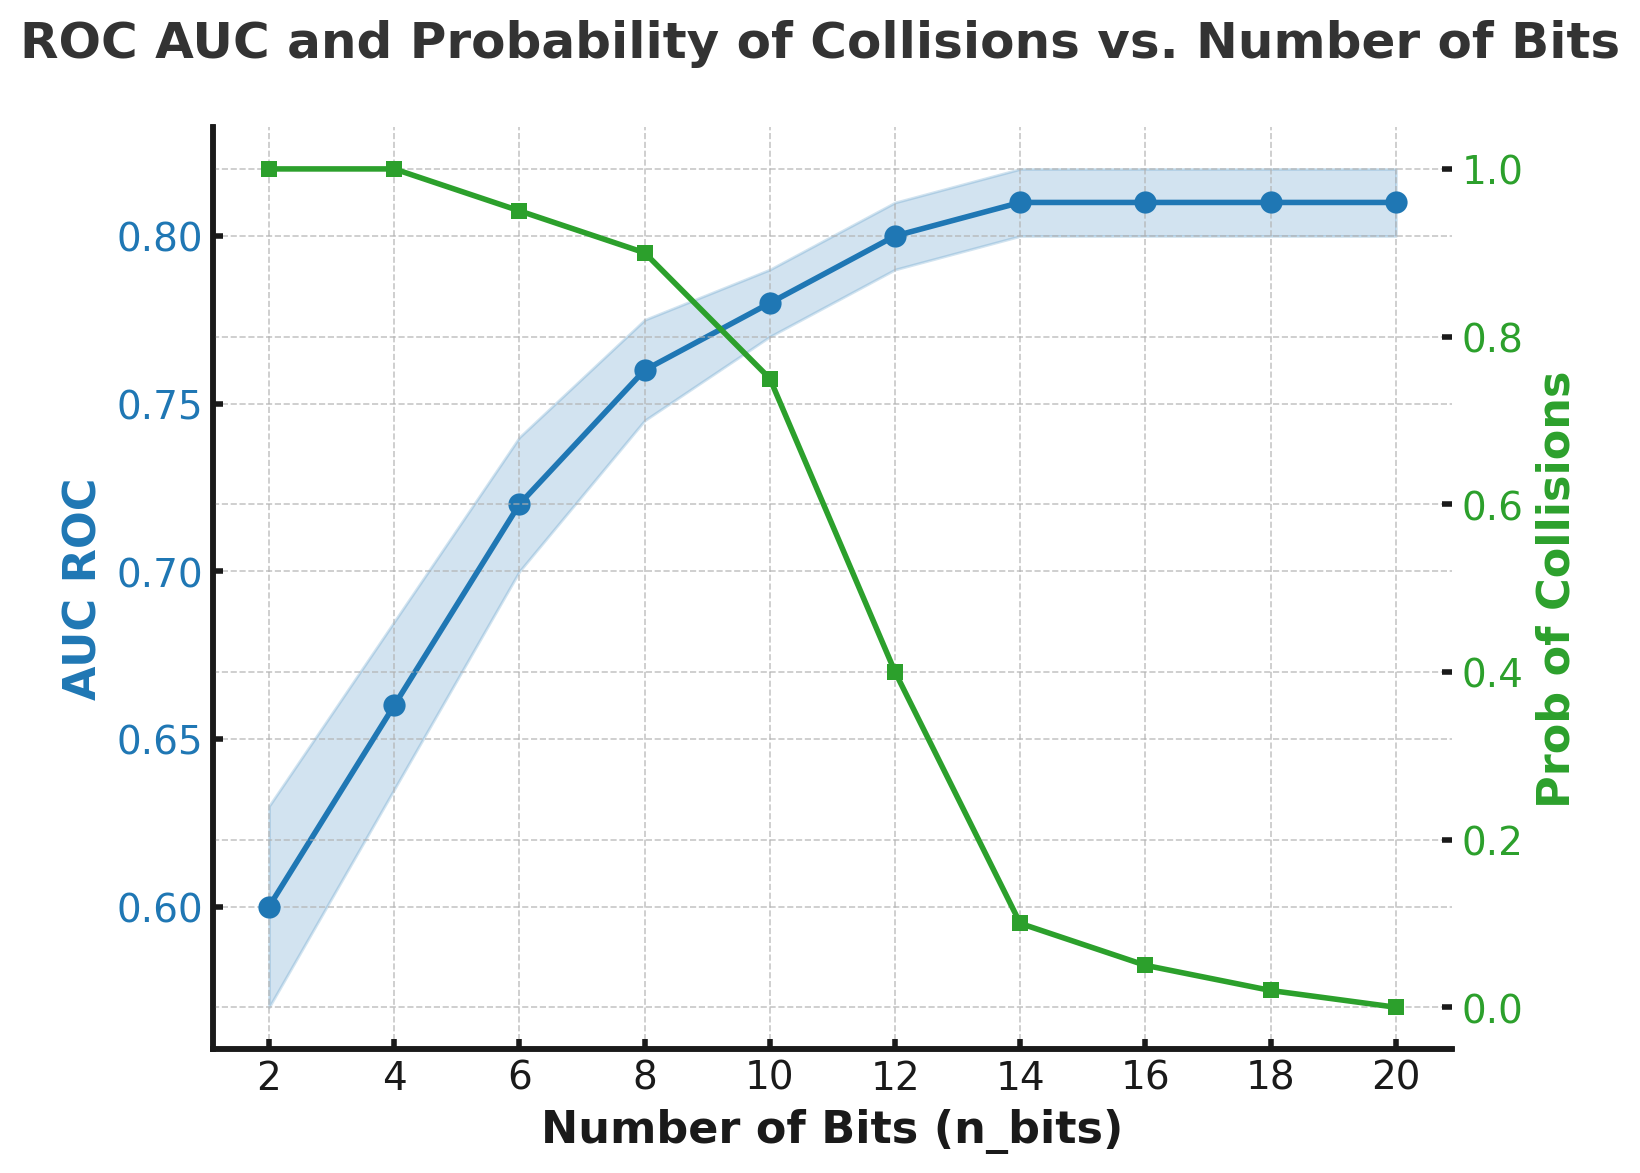
\includegraphics[
      width=\linewidth,
      trim=6 2 6 2,
      clip
    ]{images/nbit.png}
    \caption{Predictive performance vs.\ number of hash bits.}
    \label{fig:nbit-a}
  \end{subfigure}
  \hfill
  \begin{subfigure}[t]{0.50\linewidth}
    \centering
    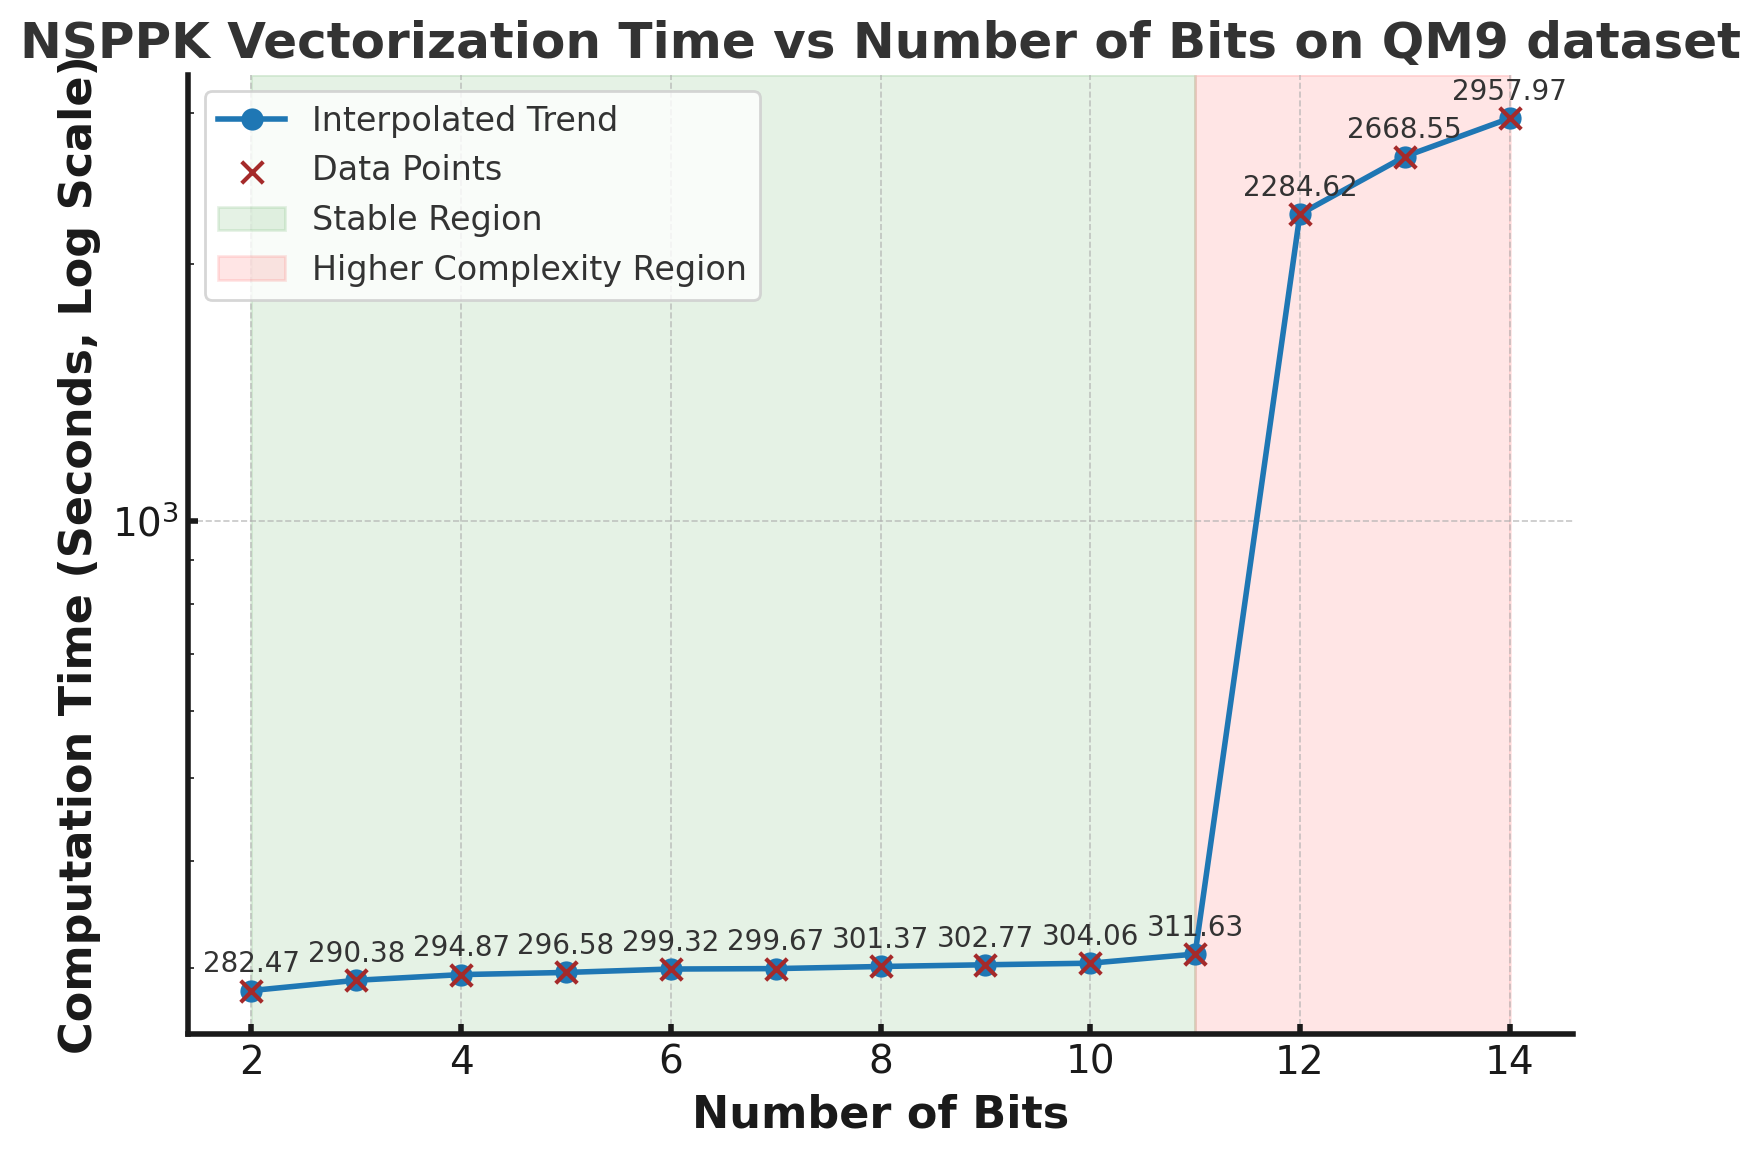
\includegraphics[width=\linewidth]{images/qm9_plot.png}
    \caption{NSPPK vectorisation time on QM9 vs.\ number of hash bits.}
    \label{fig:nsppk_qm9-a}
  \end{subfigure}

  \caption{Hash-size trade-offs: (a) predictive performance and (b) computational cost.}
  \label{fig:bits_tradeoff}
\end{figure}
\section{Diagonal Dominance and Robustness: Quantitative Analysis}
\label{sec:Diagonal}

A central pathology in similarity-based learning on graphs is the phenomenon of
\emph{diagonal dominance}. In this regime, the kernel matrix
$K\in\mathbb{R}^{N\times N}$ is dominated by its diagonal entries, with
$K_{ij}\approx 0$ for $i\neq j$. As a consequence, each graph is effectively
mapped to an isolated point, eliminating meaningful cross-graph similarity and
leading to poor generalisation and unstable optimisation. Prior work has shown
that R-convolution kernels are especially vulnerable to this effect, particularly
on graphs with high-dimensional or continuous attributes, where sparsity reduces
feature overlap even between mildly perturbed instances
\citep{gartner2003graph,shervashidze2009efficient,yanardag2015deep}.

To probe this issue, we perform a controlled robustness study. Starting from a
prototype graph $G_0$ with $n=200$ nodes, we generate a sequence of $50$
perturbed graphs $\{G_t\}_{t=1}^{50}$ through: (i) random node deletions and edge
removals while preserving connectivity, (ii) Gaussian noise injected into
five-dimensional node attributes, and (iii) a combined regime mixing structural
and attribute perturbations. For each method, we compute the full similarity
matrix $K_{ij}=k(G_i,G_j)$ across the perturbed graphs, allowing us to evaluate
both self-similarity decay and global structural preservation.

We benchmark NSPPK against five representative methods:
(1) \emph{GIN-Random} \citep{xu2019powerful}, a Graph Isomorphism Network with
random initialisation and no supervision;
(2) \emph{GraphCL} \citep{you2020graph}, a contrastive pretraining framework for
graph neural networks;
(3) \emph{InfoGraph} \citep{sun2019infograph}, an unsupervised GNN maximising
mutual information;
(4) \emph{GraphHopper} \citep{feragen2013scalable}, a shortest-path-based
kernel; and
(5) the \emph{Propagation Kernel (PK)} \citep{neumann2016propagation}, which
propagates and hashes node attributes.

Figure~\ref{fig:perturbation_panel}(a) shows the decay of normalised
self-similarity,
\[
\frac{K(G_0,G_t)}{K(G_0,G_0)},
\]
with increasing perturbation index $t$. An informative kernel should display
smooth decay: abrupt collapses indicate hypersensitivity, while nearly flat
trajectories suggest oversmoothing. GNN-based baselines such as GIN-Random and
GraphCL often remain nearly flat under structural perturbations, suggesting
insensitivity to fine-grained variation, while InfoGraph is only modestly more
responsive. In contrast, classical kernels such as GraphHopper and the
Propagation Kernel exhibit instability under attribute noise, with curves
collapsing or oscillating due to their reliance on path-based or propagation-based
dynamics. NSPPK achieves a well-calibrated, approximately monotonic decay across
all regimes, balancing sensitivity to structural changes with resilience to noise.

A complementary perspective comes from the pairwise similarity matrices in
Figure~\ref{fig:perturbation_panel}(b). Under Gaussian noise, GraphHopper and
the Propagation Kernel suffer severe diagonal dominance: bright diagonals and
small off-diagonal values indicate limited cross-graph similarity. Neural methods
such as GIN-Random, GraphCL, and InfoGraph avoid complete collapse, but often
produce oversmoothed matrices in which subtle distinctions are reduced. NSPPK
maintains dense, structured similarity patterns, avoiding diagonal collapse while
preserving discriminative variation across perturbed graphs.

\begin{figure}[t]
\centering

\begin{subfigure}[t]{0.49\linewidth}
\centering
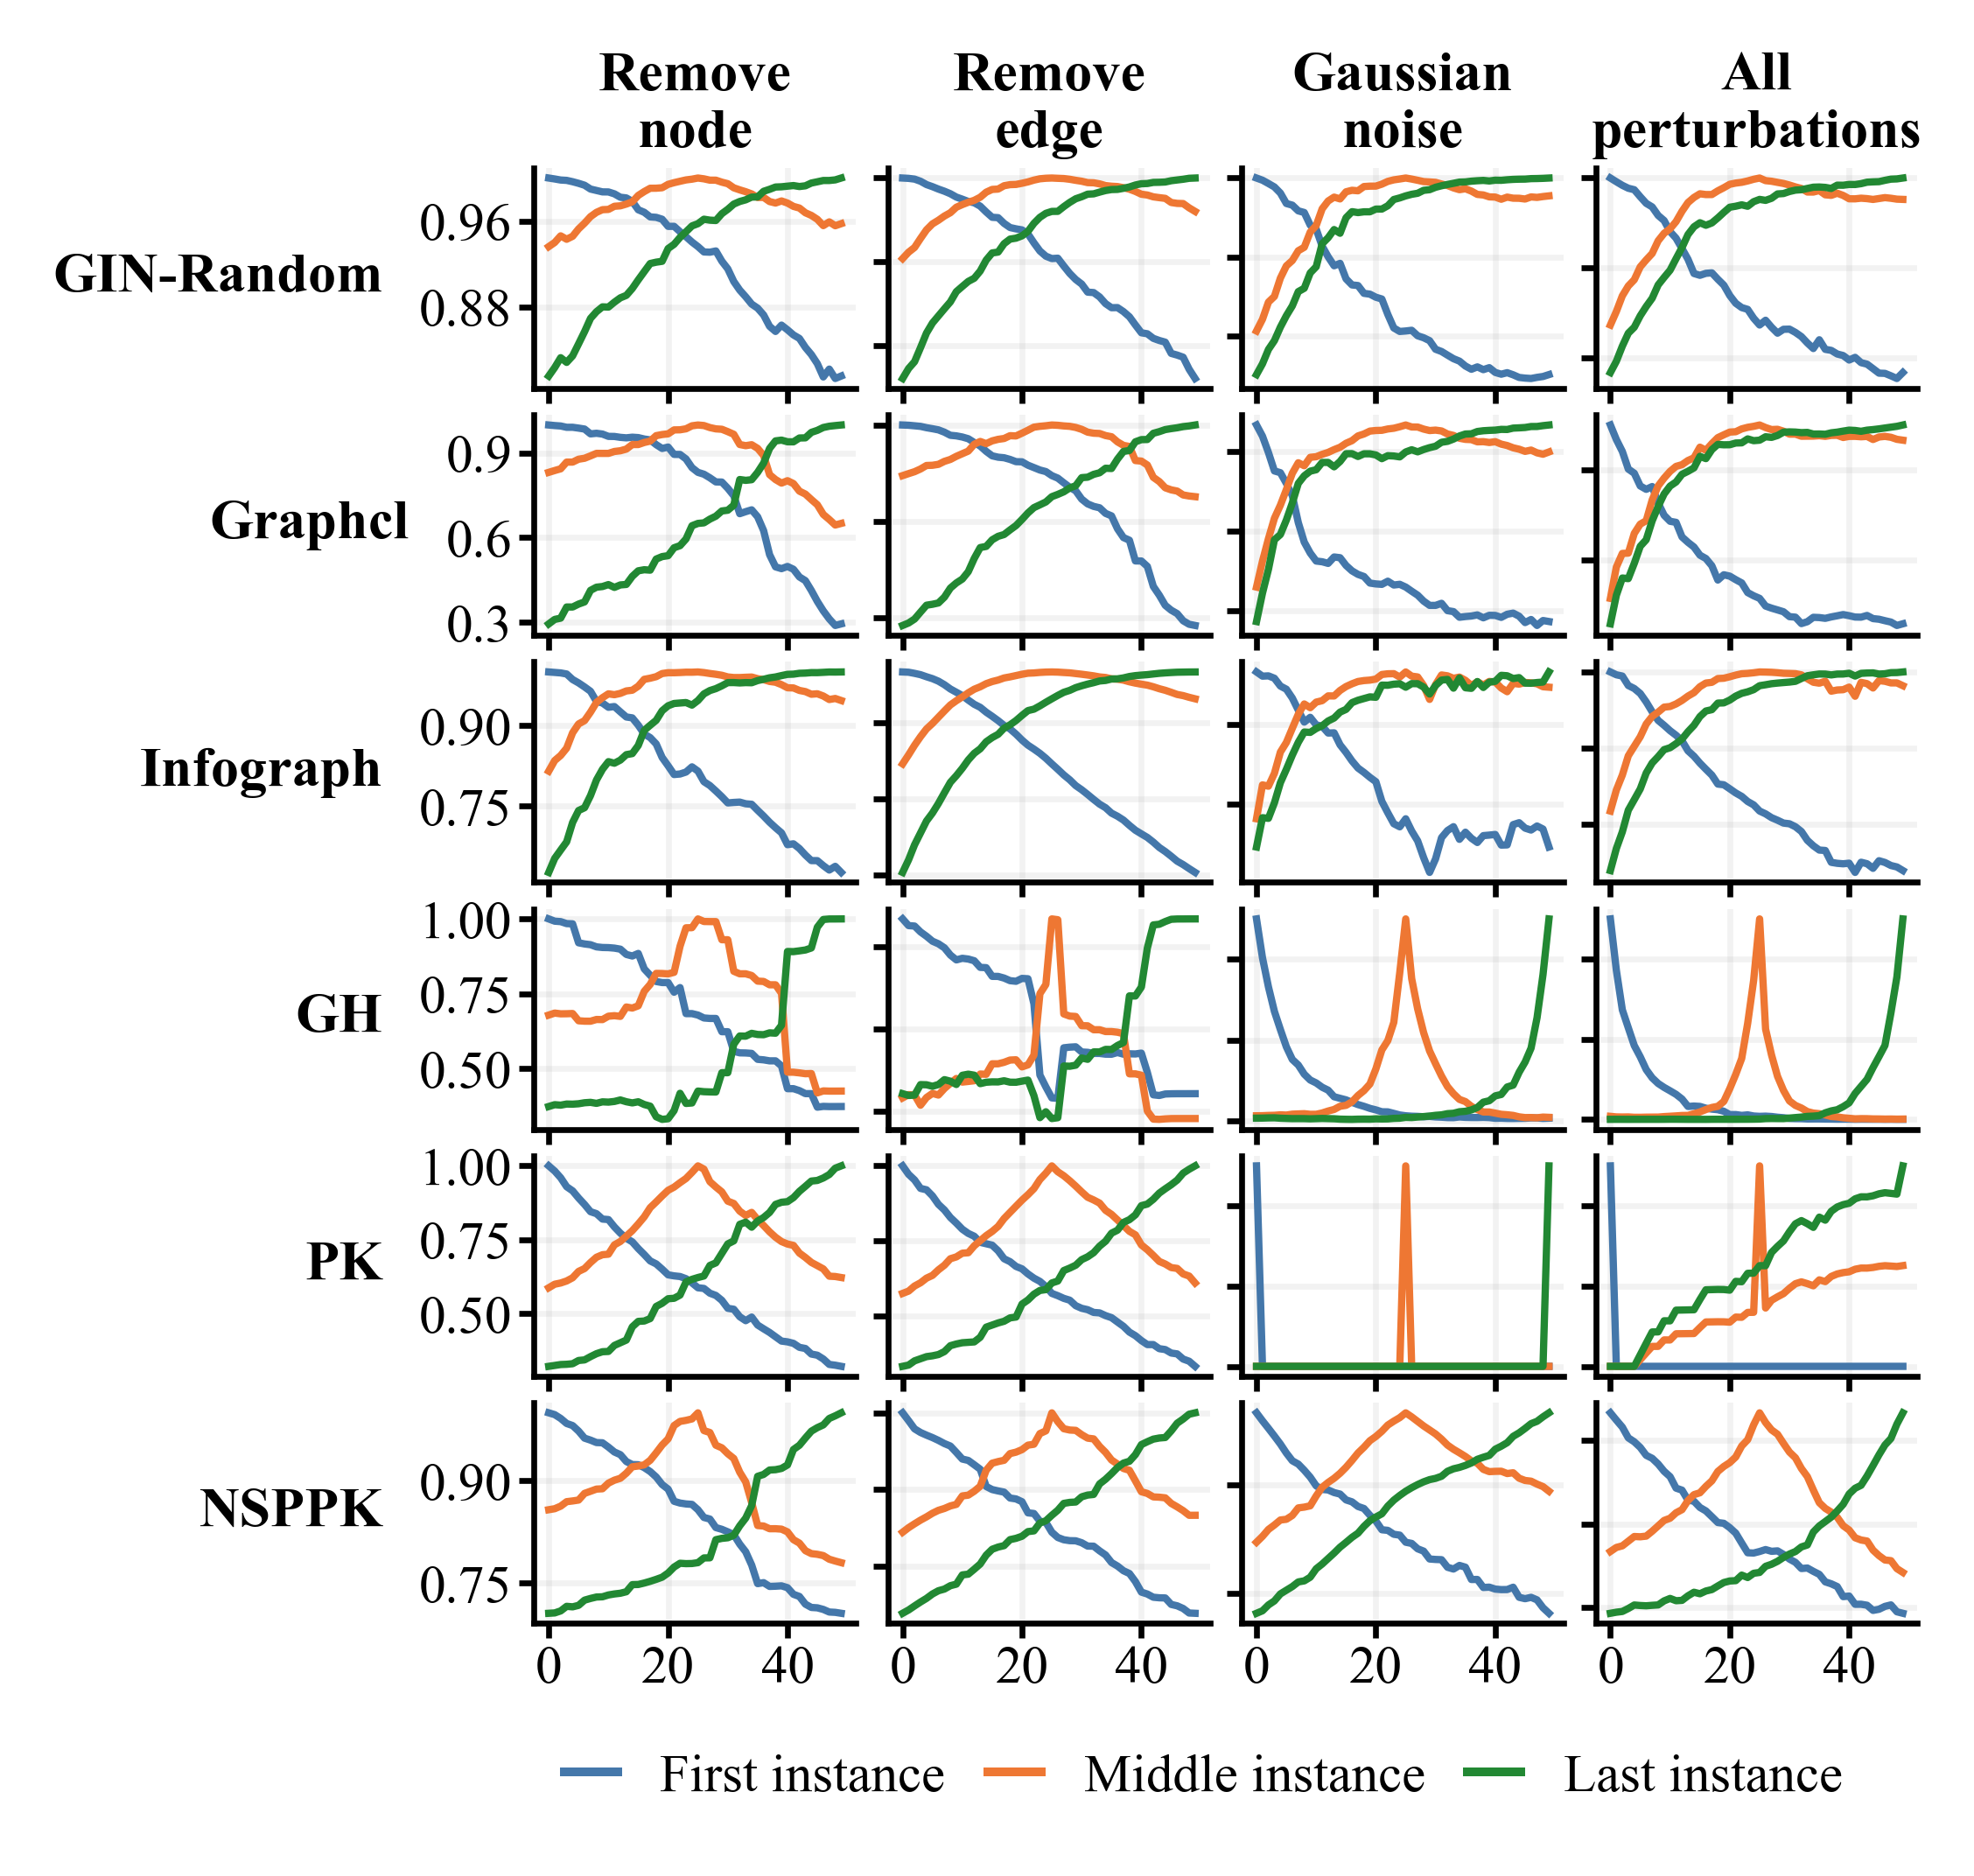
\includegraphics[width=\linewidth]{images/embedding_instance_similarity.png}
\caption{Instance similarity curves}
\label{fig:inst-curves}
\end{subfigure}
\hfill
\begin{subfigure}[t]{0.49\linewidth}
\centering
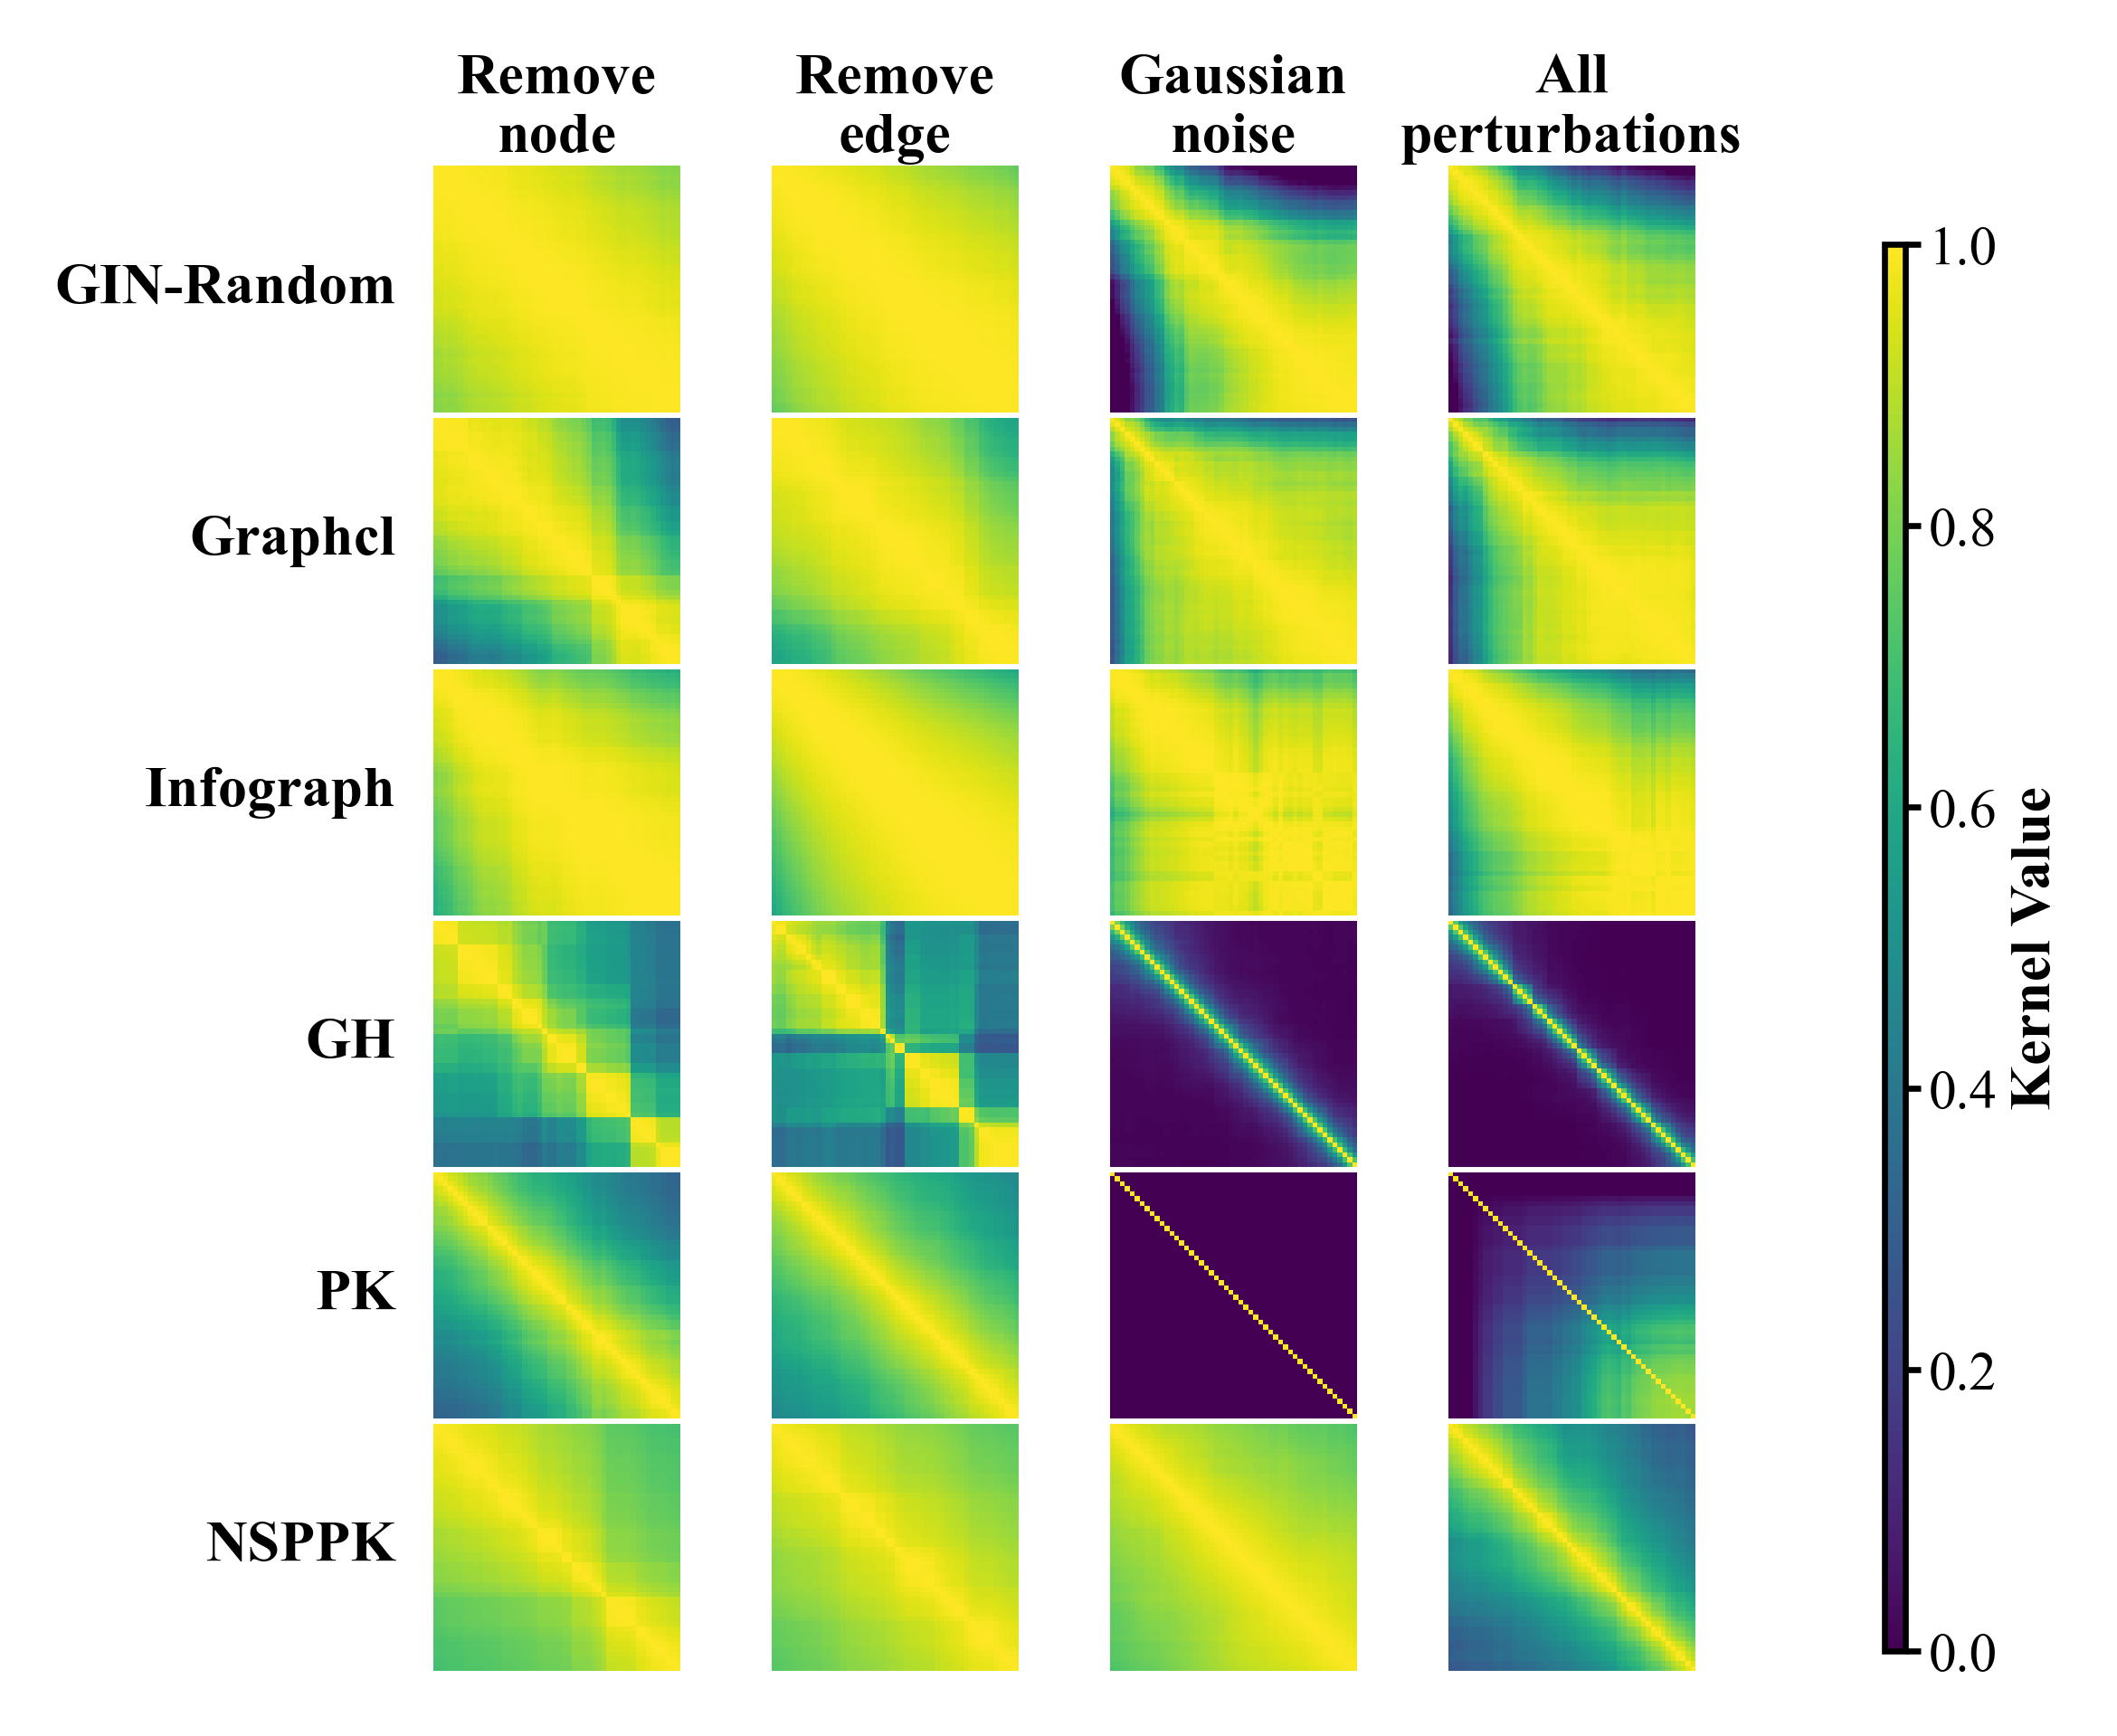
\includegraphics[width=\linewidth]{images/embedding_similarity.png}
\caption{Pairwise similarity matrices}
\label{fig:pairwise}
\end{subfigure}

\vspace{2mm}

\begin{subfigure}[t]{0.49\linewidth}
\centering
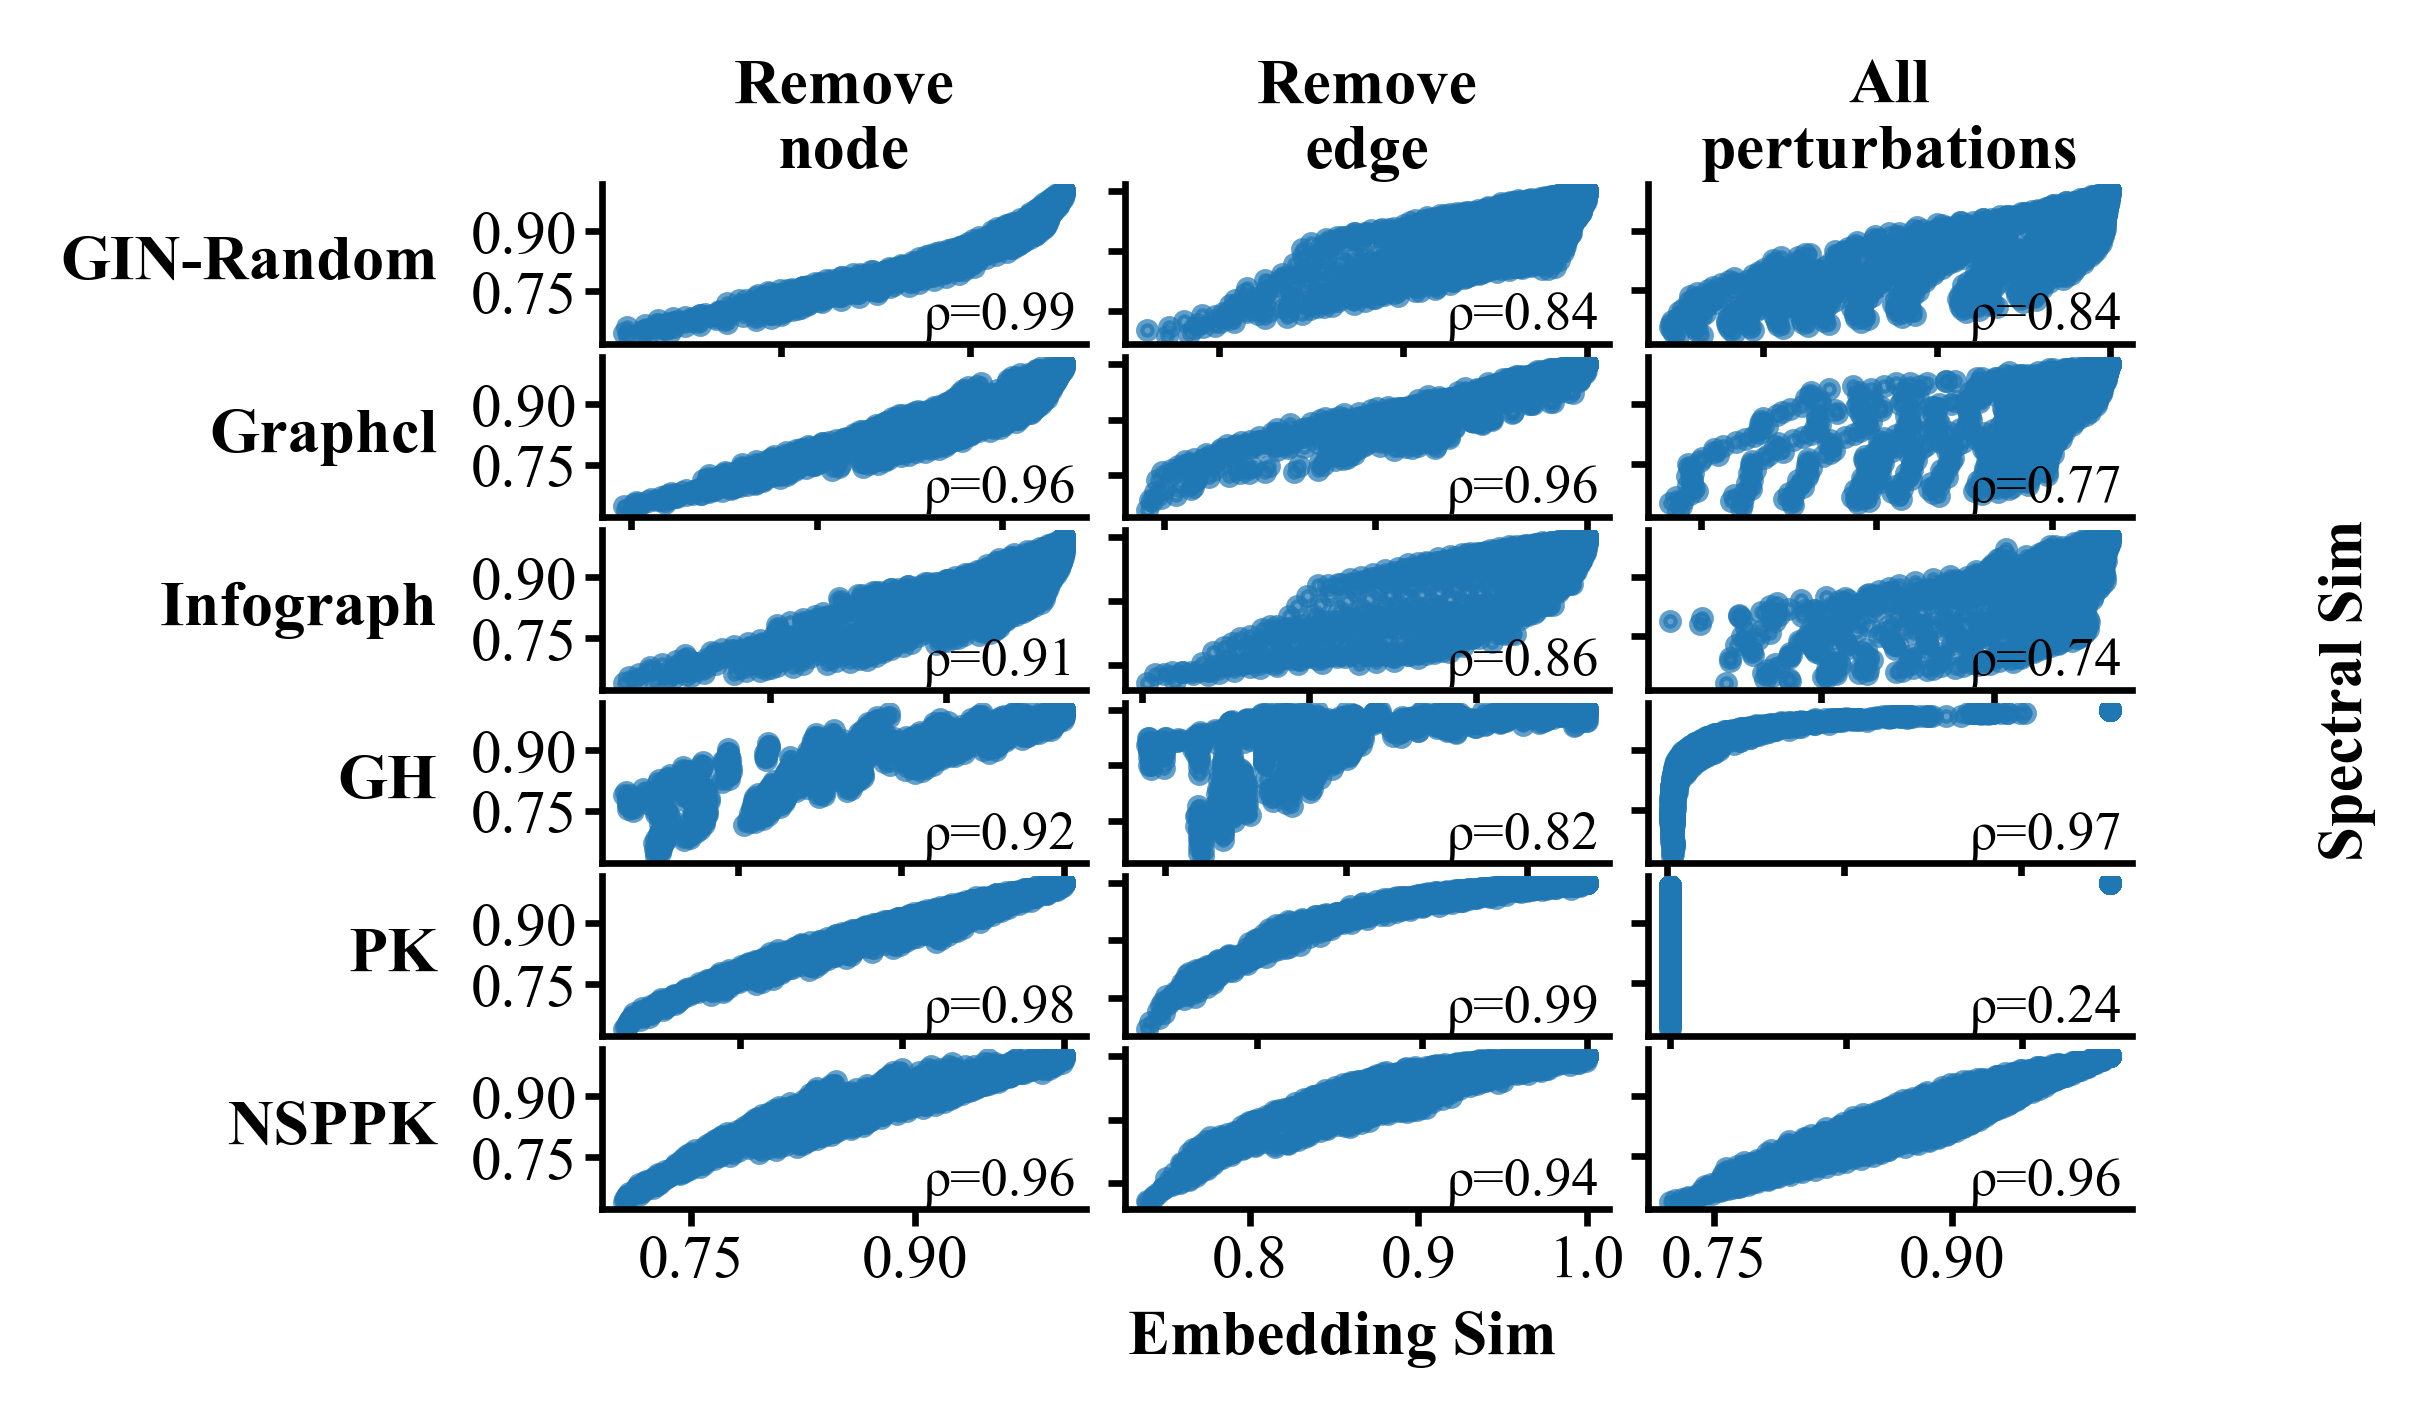
\includegraphics[width=\linewidth]{images/emb_vs_spec.png}
\caption{Embedding vs.\ spectral similarity (Spearman's $\rho$)}
\label{fig:emb-vs-spec}
\end{subfigure}
\hfill
\begin{subfigure}[t]{0.49\linewidth}
\centering
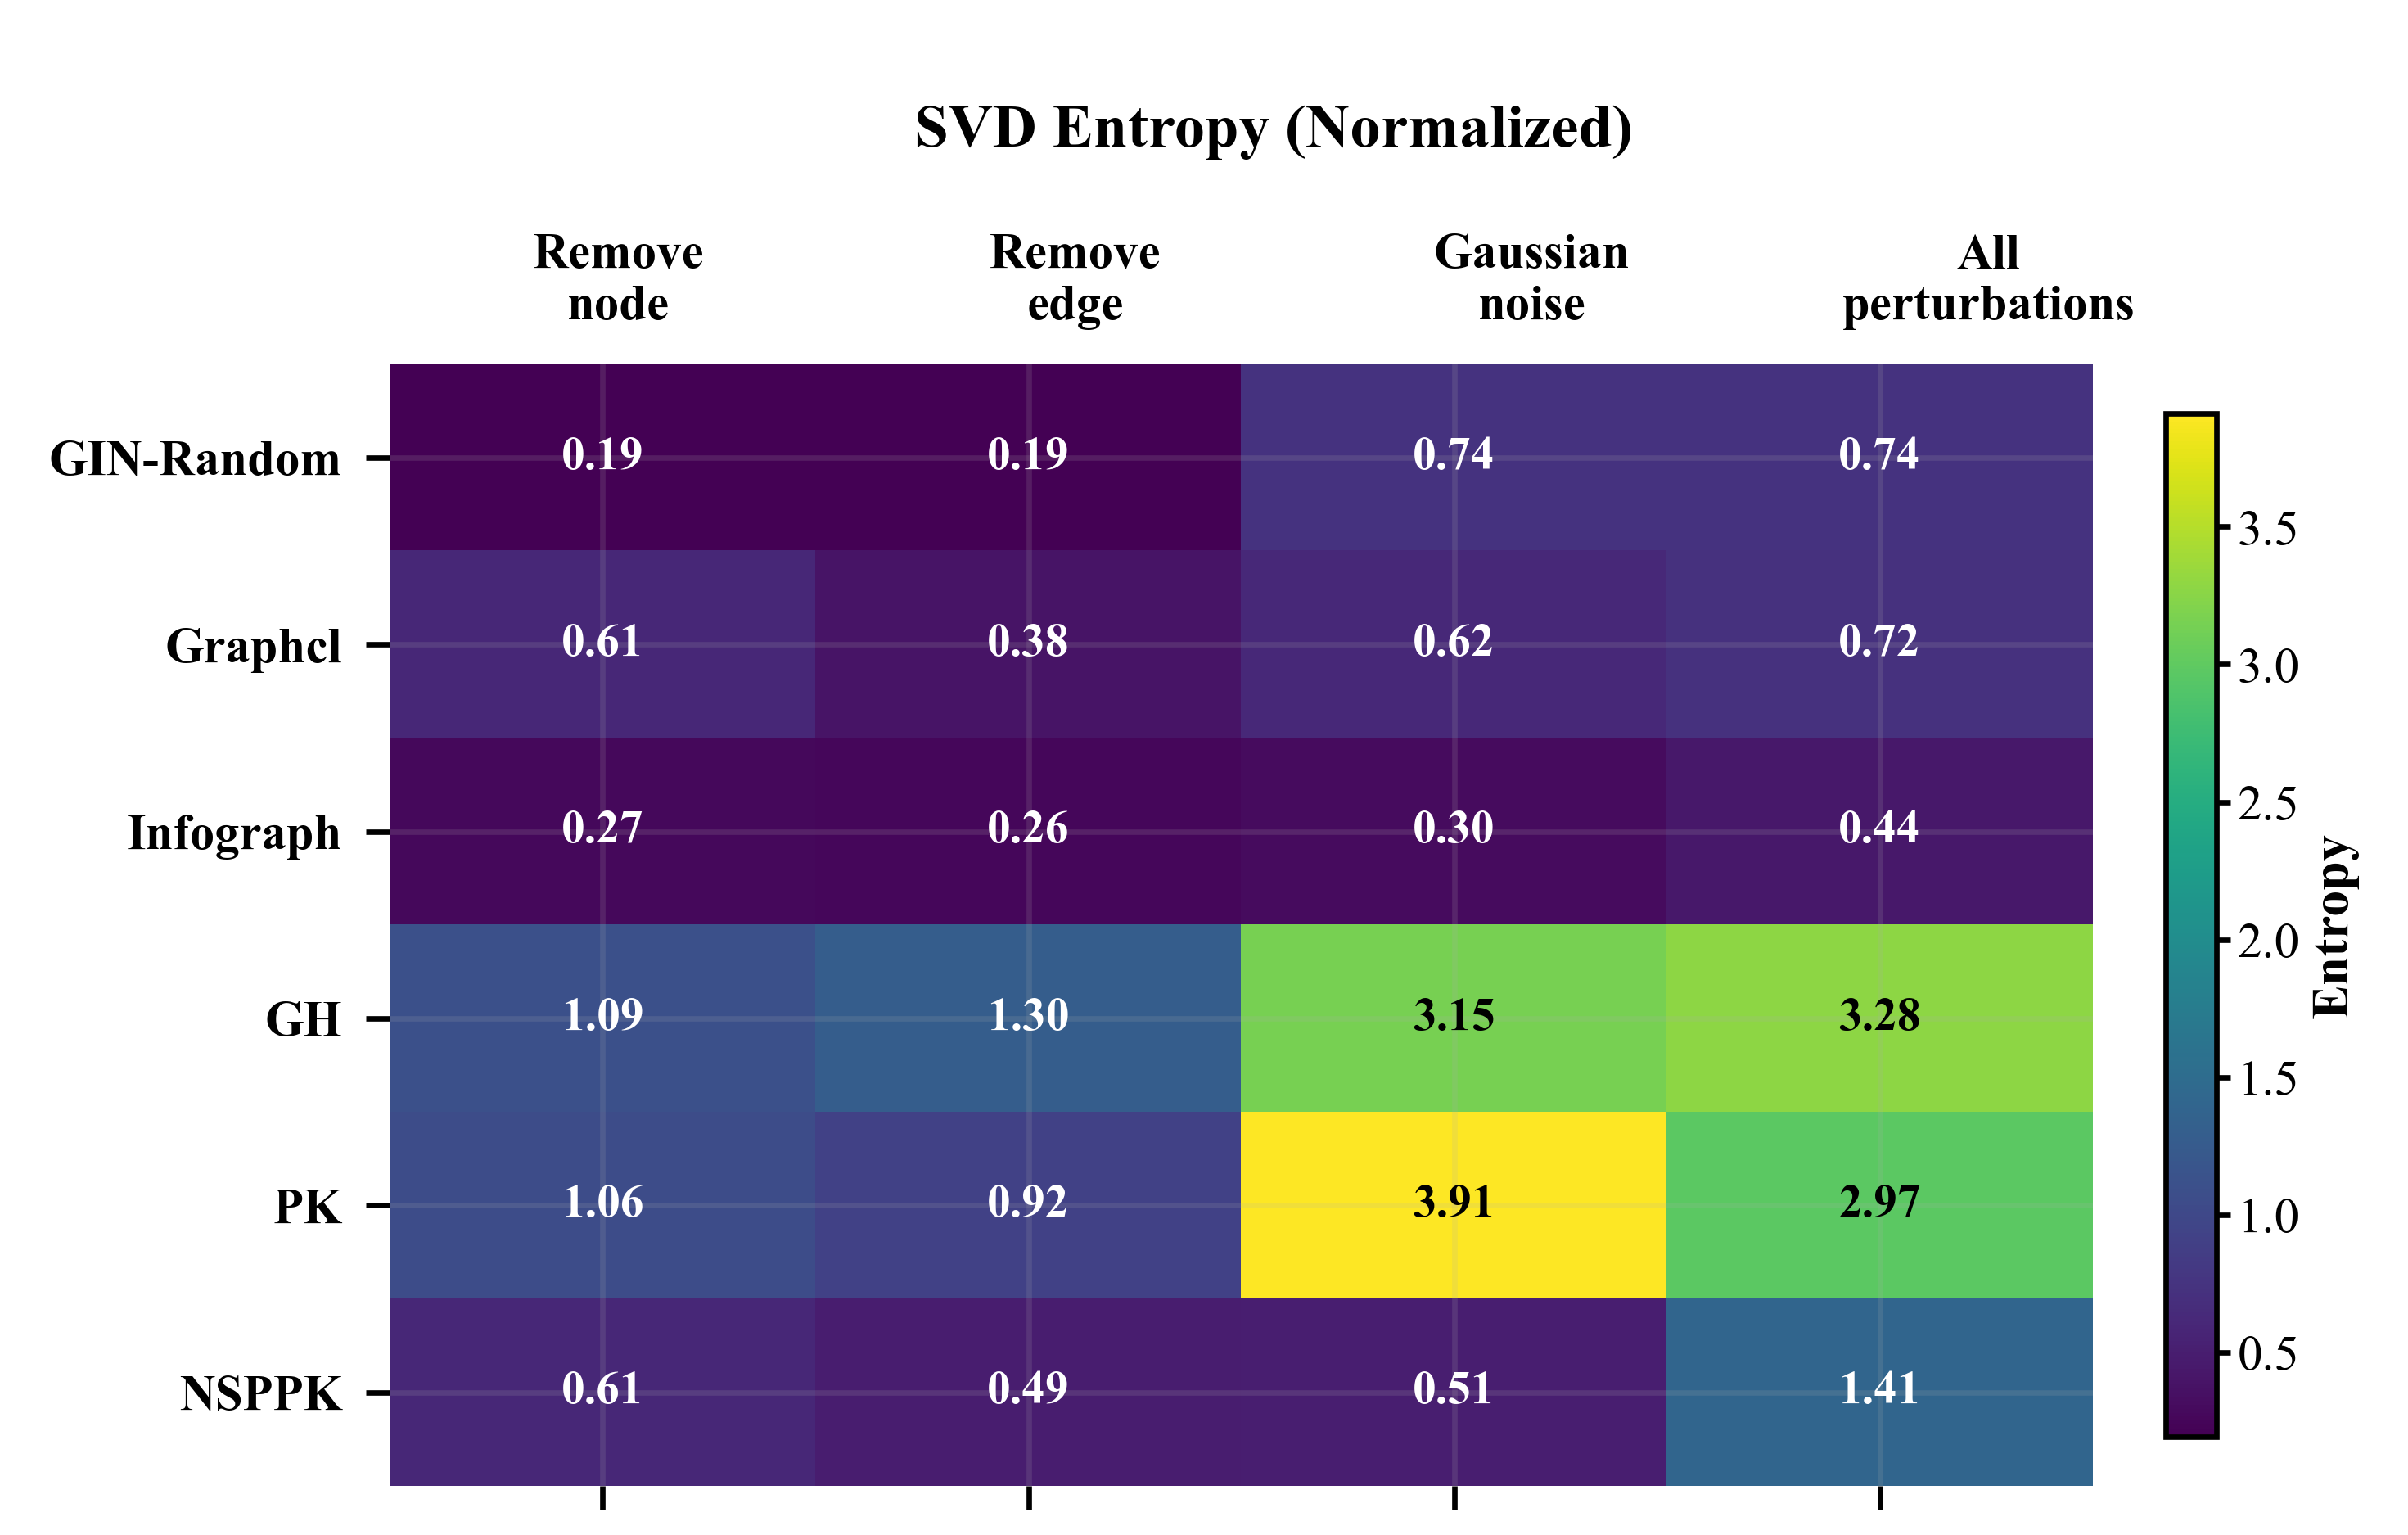
\includegraphics[width=\linewidth]{images/svd_entropy.png}
\caption{SVD entropy of similarity matrices}
\label{fig:svd-entropy}
\end{subfigure}

\caption{\textbf{Unified robustness analysis of graph similarity methods under perturbations.}
(a) Decay of self-similarity across perturbations.
(b) Pairwise similarity matrices showing diagonal dominance in baselines versus NSPPK.
(c) Correlation between kernel similarity and spectral similarity (Spearman $\rho$).
(d) SVD entropy of similarity matrices. NSPPK preserves stable, meaningful similarity structure, avoiding diagonal collapse.}
\label{fig:perturbation_panel}

\end{figure}

We further assess \emph{spectral alignment} by measuring the Spearman correlation
$\rho$ between kernel similarities and Laplacian spectral similarity
(Figure~\ref{fig:perturbation_panel}(c)). High $\rho$ indicates embeddings that
respect the intrinsic geometry of the graph family. NSPPK consistently achieves
high alignment across perturbations, while GNN-based methods perform
competitively but degrade under mixed noise, consistent with known oversmoothing
effects~\citep{kipf2017semi,oono2019graph,rong2020dropedge,balcilar2021analyzing}.
Classical kernels fare worse: the Propagation Kernel degrades under attribute
perturbations, and GraphHopper shows inconsistent alignment across regimes.

Finally, we quantify \emph{global expressivity} using normalised SVD entropy of
the similarity matrix,
\[
H_{\mathrm{SVD}} = -\sum_i \lambda_i \log \lambda_i.
\]
where $\{\lambda_i\}$ are the singular values of $K$ normalised to unit sum
(Figure~\ref{fig:perturbation_panel}(d)). Low entropy indicates spectral
degeneracy, where only a few singular directions explain most of the variation;
very high entropy may instead reflect instability or noise. Classical kernels can
exhibit unstable entropy under Gaussian noise, suggesting sensitivity to noisy
directions rather than genuine structural diversity. GNN baselines tend to yield
lower entropy, indicating stable but potentially under-expressive embeddings.
NSPPK maintains a high but stable entropy profile, reflecting a richer
similarity structure without diagonal collapse.

Taken together, these results show that NSPPK mitigates diagonal dominance while
preserving robustness and expressivity. Unlike prior kernels
\citep{shervashidze2009efficient,yanardag2015deep,neumann2016propagation} and
GNN methods \citep{xu2019powerful,yi2022graph,sun2019infograph}, which are prone
to either instability or oversmoothing under perturbation, NSPPK provides stable,
interpretable embeddings that respect spectral geometry and maintain
discriminative power.

\section{Experiments}
\label{sec:experiments}

\subsection{Small-Scale Datasets}
\label{sec:small_datasets}

We evaluate NSPPK against kernel and neural baselines on six node-attributed
graph classification benchmarks: \emph{ENZYMES},
\emph{PROTEINS\_full}, \emph{BZR}, \emph{COX2}, \emph{DHFR}, and
\emph{SYNTHETICnew}. Detailed dataset descriptions and summary statistics are
provided in Appendix~\ref{appendix:datasets}.


\textbf{Baselines.}
Kernel methods: GraphHopper (GH)~\citep{feragen2013scalable}, Propagation Kernel (PK)~\citep{neumann2016propagation}, Subgraph Matching (SM)~\citep{kriege2012subgraph}, Multiscale Laplacian (ML)~\citep{kondor2016multiscalelaplaciangraphkernel}, Shortest Path (SP)~\citep{borgwardt2005shortest}, HSSPK-SP/WL~\citep{morris2016fasterkernelsgraphscontinuous}, WWL~\citep{togninalli2019wasserstein}, linearFGW~\citep{nguyen2023linearfgw}, and NP~\citep{fang2023neighborhoodpreserving}, plus discretised NSPPK and WL.
All kernels use SVM classifiers (LIBSVM~\citep{chang2011libsvm}).

\textbf{Neural baselines}: DGCNN~\citep{zhang2018endtoend}, GraphSAGE~\citep{hamilton2017graphsage}, InfoGraph~\citep{sun2019infograph}, GIN~\citep{xu2019powerful}, GraphCL~\citep{you2020graph}, AttentiveFP (FNP)~\citep{gasteiger2020directional}, PNA~\citep{corso2020pna}, and PDF~\citep{yang2023bettergraphrepresentationlearning}.

\textbf{Protocol.}
We follow the fair evaluation setup of~\citep{errica2020fair}: 10-fold cross-validation with 10\% validation from training data.
Kernels: SVM with $C$ tuned on validation; multiple hyperparameter configurations tested; kernel computation times reported for best models.
GNNs: trained up to 1000 epochs with early stopping; tuned via validation.
The hyperparameter grids used for model selection for both neural and kernel baselines are reported in Appendix~\ref{appendix:hyperparameters}.

\textbf{Controls.}
We also test (i) \emph{attributes only}, where graphs are represented by summed node attributes, and (ii) \emph{structure only}, where attributes are removed (Appendix~\ref{appendix:no_attr}).

 \textbf{NSPPK}: fixed configuration across all datasets ($R{=}1,D{=}4,R'{=}1$, 16-bit hashing); no per-dataset tuning.
For comparison with kernels we use LIBSVM, and for GNNs we use NSPPK features with XGBoost.
All kernel runtimes, including NSPPK, are measured on a single CPU core for comparability.

\textbf{Runtime.}
Kernel methods run on a single CPU core; GNNs run on CPUs with library-level multithreading. All experiments used a SLURM-managed cluster with NVIDIA A100 GPUs, Intel Xeon Gold 5317 CPUs (24 cores), and 64 GB RAM. Kernels exceeding 24h per fold are reported as timeouts.



\begin{table}[t]
\centering
\caption{Classification accuracy (\%) with node attributes (+) and average rank.}
\label{tab:with_attr}
\scriptsize
\setlength{\tabcolsep}{3.2pt}
\begin{adjustbox}{max width=\textwidth}
\begin{tabular}{lccccccc}
\toprule
\textbf{Method} & \makecell{\textbf{SYNTHETIC}\\\textbf{new}} & \textbf{DHFR} & \textbf{BZR} & \textbf{COX2} & \textbf{ENZYMES} & \textbf{PROTEINS} & \textbf{Avg Rank} \\
\midrule
SM                      & \TO & \TO & \mps{83.96}{3.85} & \mps{78.81}{4.49} & \TO & \TO & ~8* \\
SP                      & \TO & \TO & \TO & \TO & \TO & \TO & -- \\
ML                      & \mps{50.33}{9.00} & \mps{78.57}{4.21} & \mps{82.96}{5.24} & \mps{77.53}{5.53} & \mps{36.33}{4.33} & \mps{72.06}{3.60} & 10.25 \\
PK                      & \mps{54.33}{10.11} & \mps{60.98}{0.48} & \mps{78.77}{1.01} & \mps{78.16}{8.07} & \mps{20.67}{2.70} & \mps{59.70}{0.16} & 12.58 \\
HSPPK\_WL               & \mps{60.33}{6.74} & \mps{77.38}{5.44} & \mps{85.67}{3.46} & \mps{80.30}{4.67} & \mps{60.17}{6.26} & \mps{72.96}{4.84} & 5.75\\
HSPPK\_SP               & \mps{57.00}{7.81} & \mps{77.40}{3.85} & \mps{84.49}{5.04} & \mps{80.31}{5.70} & \mps{58.50}{5.55} & \mps{68.55}{5.24} & 7.17 \\
GH                      & \mps{77.33}{7.42} & \mps{78.19}{5.47} & \mps{85.94}{5.17} & \mps{78.90}{2.95} & \mps{66.50}{6.17} & \mps{72.06}{3.64} & 4.75 \\
NP                      & \textbf{\mps{99.00}{2.13}} & \mps{80.42}{4.57} & \mps{86.18}{5.53} & \mps{78.16}{4.47} & \mps{43.00}{5.76} & \mps{64.62}{5.13} & 6.58 \\
linearFGW-RAW           & \mps{62.00}{8.46} & \mps{60.85}{3.75} & \mps{76.34}{5.68} & \mps{77.93}{3.68} & \mps{56.67}{7.07} & \mps{69.47}{0.91} & 10.83 \\
linearFGW-WL1           & \mps{72.33}{8.70} & \mps{59.94}{4.11} & \mps{78.52}{3.99} & \mps{72.13}{7.40} & \mps{47.00}{4.70} & \mps{59.66}{0.38} & 12.83 \\
linearFGW-WL2           & \mps{71.33}{7.48} & \mps{57.82}{5.48} & \mps{78.51}{2.98} & \mps{75.16}{3.34} & \mps{41.00}{7.57} & \mps{59.75}{0.43} & 13.00 \\
WL (disc.)              & \mps{88.33}{5.63} & \mps{77.26}{5.81} & \mps{83.71}{4.83} & \mps{77.10}{5.59} & \mps{50.67}{7.03} & \mps{71.16}{4.03} & 8.75 \\
WLOA                    & \mps{85.33}{5.62} & \mps{75.00}{3.23} & \mps{84.20}{4.47} & \mps{74.54}{5.40} & \mps{66.33}{5.21} & \mps{71.16}{1.97} & 8.08 \\
WWL                     & \mps{58.33}{7.78} & \mps{77.12}{3.58} & \mps{86.45}{4.50} & \mps{79.03}{3.84} & \textbf{\mps{73.67}{5.26}} & \textbf{\mps{77.18}{5.27}} & 4.83 \\
NSPDK (disc.)           & \mps{96.33}{3.14} & \mps{82.93}{5.56} & \mps{85.70}{3.90} & \mps{80.30}{4.15} & \mps{52.67}{4.67} & \mps{72.87}{1.51} & 4.42 \\
\rowcolor{gray!10}
NSPPK (ours)            & \textbf{\mps{99.00}{1.52}} & \textbf{\mps{82.95}{4.57}} & \textbf{\mps{87.17}{3.58}} & \mps{81.16}{2.30} & \mps{60.50}{5.38} & \mps{74.66}{3.81} & \textbf{1.75} \\
\midrule
\emph{Attributes only}  & \mps{54.33}{9.55} & \mps{60.98}{4.80} & \mps{78.77}{1.01} & \mps{78.16}{8.07} & \mps{55.67}{5.38} & \mps{62.80}{2.52} & 11.50 \\
\bottomrule
\end{tabular}
\end{adjustbox}

\vspace{0.5ex}
{\footnotesize\emph{Note:} ``Attributes only'' participates in Avg Rank like any other method.}
\end{table}

% ========================= NEURAL NETS — WITH ATTRIBUTES =========================
\begin{table}[t]
\centering
\caption{Neural networks: classification accuracy (\%) with node attributes (+) and Avg Rank.}
\label{tab:nn_with_attr}
\scriptsize
\setlength{\tabcolsep}{3.2pt}
\begin{adjustbox}{max width=\textwidth}
\begin{tabular}{lccccccc}
\toprule
\textbf{Method} & \textbf{\makecell{SYNTHETIC\\new}} & \textbf{DHFR} & \textbf{BZR} & \textbf{COX2} & \textbf{ENZYMES} & \textbf{PROTEINS} & \textbf{Avg Rank} \\
\midrule
DGCNN                & \mps{46.67}{5.63} & \mps{68.77}{5.52} & \mps{79.40}{3.32} & \mps{77.15}{0.06} & \mps{33.33}{9.37} & \mps{73.86}{3.56} & 10.58 \\
GraphSAGE            & \mps{76.67}{7.70} & \mps{76.46}{4.13} & \mps{83.70}{4.44} & \mps{80.93}{0.07} & \mps{65.00}{5.73} & \mps{75.02}{3.29} & 4.42 \\
InfoGraph            & \mps{65.00}{16.05} & \mps{73.01}{6.03} & \mps{79.01}{3.42} & \mps{77.77}{14.20} & \mps{53.33}{7.84} & \mps{66.37}{6.25} & 7.25 \\
GIN                  & \mps{83.67}{5.92} & \mps{76.85}{7.23} & \mps{84.17}{6.14} & \mps{81.80}{6.14} & \textbf{\mps{68.30}{5.43}} & \mps{62.10}{5.26} & 4.33\\
GraphCL              & \mps{67.00}{9.48} & \mps{80.34}{6.95} & \mps{84.17}{3.62} & \mps{80.34}{6.95} & \mps{48.17}{6.93} & \mps{75.82}{2.73} & 5.17 \\
GNN                  & \mps{64.67}{7.92} & \mps{76.59}{6.97} & \mps{85.66}{4.60} & \mps{79.92}{7.08} & \mps{65.17}{8.41} & \mps{66.57}{6.10} & 5.50 \\
FNP                  & \mps{53.33}{11.16} & \mps{70.76}{3.99} & \mps{79.49}{3.94} & \mps{78.22}{7.01} & \mps{32.17}{12.98} & \mps{70.17}{3.15} & 9.42 \\
PNA                  & \mps{55.67}{20.66} & \mps{61.50}{5.42} & \mps{79.01}{4.33} & \mps{78.22}{7.02} & \mps{20.83}{7.12} & \mps{75.11}{3.60} & 8.17 \\
PDF                  & \mps{97.67}{2.60} & \mps{77.37}{4.50} & \mps{83.68}{3.81} & \mps{82.23}{7.00} & \mps{65.00}{4.65} & \mps{72.14}{4.48} & 3.75 \\
\rowcolor{gray!10}
NSPPK feat.\ (XGBoost) & \textbf{\mps{98.67}{2.21}} & \textbf{\mps{83.74}{4.14}} & \textbf{\mps{88.66}{2.89}} & \textbf{\mps{82.90}{4.39}} & \mps{60.17}{6.30} & \textbf{\mps{77.37}{4.80}} & \textbf{1.67} \\
\midrule
\emph{Attributes only} & \mps{54.33}{9.55} & \mps{60.98}{ 4.80}& \mps{78.77}{1.01} & \mps{78.16}{8.07} & \mps{55.67}{5.38} & \mps{62.80}{2.52} & 7.75 \\
\bottomrule
\end{tabular}
\end{adjustbox}
\end{table}


\subsubsection{Runtime and Efficiency}
\label{sec:runtime}


Against \emph{kernels}, NSPPK achieves the best accuracy on four out of six
benchmarks (\emph{SYNTHETICnew}, \emph{BZR}, \emph{COX2},\emph{DHFR}) and the best overall
average rank (1.75 vs >4 for other kernels).
Under a conservative single-core evaluation setting, NSPPK delivers a favourable
efficiency--accuracy trade-off among kernel methods. Very lightweight baselines
such as GraphCL or PNA achieve lower runtimes (average rank $7.50$), but NSPPK
remains substantially more efficient than expressive graph kernels such as GH or
HSPPK, while consistently achieving higher predictive accuracy. When paired with
XGBoost, NSPPK delivers the strongest overall accuracy among kernel-based
methods.
Detailed runtime measurements are reported in
Tables~\ref{tab:with_attr_runtime_kernels} and~\ref{tab:with_attr_runtime_nns}.
Overall, NSPPK provides a favourable efficiency--accuracy trade-off,
achieving substantially higher accuracy than lightweight kernels while
remaining significantly more efficient than high-expressivity methods.
Additional visualizations of the accuracy--time trade-off across datasets
are provided in Appendix~\ref{appendix:tradeoff}.


\begin{table}[H]
\centering
\caption{Runtime (seconds) \textbf{with} node attributes (\textbf{lower is better}).}
\scriptsize
\label{tab:with_attr_runtime_kernels}
\setlength{\tabcolsep}{3.5pt}
\begin{adjustbox}{max width=\textwidth}
\begin{tabular}{lcccccccc}
\toprule
\textbf{Method} & \makecell{\textbf{SYNTHETIC}\\\textbf{NEW}} & \textbf{DHFR} & \textbf{BZR} & \textbf{COX2} & \textbf{ENZYMES} & \textbf{PROTEINS} & \textbf{Avg} & \textbf{Rank}\\
\midrule
SM & \TO & \TO & 12274.00\,s & 25927.96\,s & \TO & \TO & 19100.98\,s & 15.00\\
ML & 1777.93\,s & 1361.75\,s & 849.20\,s & 1155.49\,s & 1295.99\,s & 3628.70\,s & 1678.18\,s & 13.83\\
PK & 1.81\,s & 2.82\,s & 0.79\,s & 1.13\,s & 3.14\,s & 4.48\,s & 2.36\,s & \textbf{1.33}\\
HSPPK\_WL & 49.54\,s & 51.49\,s & 8.63\,s & 16.38\,s & 25.20\,s & 89.90\,s & 40.19\,s & 9.33\\
HSPPK\_SP & 249.75\,s & 63.1\,s & 16.52\,s & 29.22\,s & 28.35\,s & 119.32\,s & 84.38\,s & 11.00\\
GH & 242.05\,s & 318.8\,s & 112.43\,s & 132.63\,s & 365.25\,s & 3647.21\,s & 803.06\,s & 13.00\\
NP & 41.57\,s & 217.54\,s & 42.32\,s & 69.80\,s & 17.69\,s & 49.58\,s & 73.08\,s & 10.00\\
linearFGW-RAW & 6.82\,s & 22.14\,s & 6.63\,s & 9.84\,s & 8.73\,s & 69.67\,s & 20.64\,s & 5.50\\
linearFGW-WL1 & 6.94\,s & 22.58\,s & 5.89\,s & 10.75\,s & 8.29\,s & 67.19\,s & 20.27\,s & 5.50\\
linearFGW-WL2 & 5.95\,s & 25.23\,s & 7.02\,s & 10.92\,s & 10.26\,s & 71.63\,s & 21.84\,s & 6.50\\
WL (disc.) & 12.33\,s & 0.21\,s & 4.00\,s & 14.00\,s & 9.00\,s & 20.00\,s & 9.92\,s & 5.00\\
WLOA & 0.99\,s & 10.49\,s & 0.83\,s & 3.27\,s & 4.24\,s & 12.67\,s & 5.42\,s & 2.75\\
WWL & 29.96\,s & 105.03\,s & 14.71\,s & 40.89\,s & 32.54\,s & 134.95\,s & 59.68\,s & 10.67\\
NSPDK (disc.) & 6.50\,s & 10.49\,s & 4.69\,s & 2.64\,s & 3.18\,s & 6.13\,s & 5.61\,s & 3.08\\
\rowcolor{gray!10}
\textbf{NSPPK (ours)} & 34.81\,s & 36.19\,s & 12.75\,s & 12.75\,s & 26.45\,s & 5.73\,s & 21.45\,s & 7.50\\
\bottomrule
\end{tabular}
\end{adjustbox}
\end{table}

% ========================= RUNTIMES: NEURAL (WITH ATTRS) =========================
% ========================= RUNTIMES: NEURAL (WITH ATTRS) =========================
\begin{table}[H]
\centering
\caption{Neural runtimes (seconds) \textbf{with} node attributes (\textbf{lower is better}).}
\label{tab:with_attr_runtime_nns}
\scriptsize
\setlength{\tabcolsep}{3.5pt}
\begin{adjustbox}{max width=\textwidth}
\begin{tabular}{lcccccccc}
\toprule
\textbf{Method} & \makecell{\textbf{SYNTHETIC}\\\textbf{NEW}} & \textbf{DHFR} & \textbf{BZR} & \textbf{COX2} & \textbf{ENZYMES} & \textbf{PROT} & \textbf{Avg} & \textbf{Rank}\\
\midrule
DGCNN & 443.59\,s & 2956.95\,s & 304.88\,s & 704.74\,s & 948.88\,s & 1512.29\,s & 1145.22\,s & 9.83\\
GraphSAGE & 139.94\,s & 101.76\,s & 175.30\,s & 118.97\,s & 317.84\,s & 394.02\,s & 174.79\,s & 7.33\\
InfoGraph & 39.25\,s & 163.79\,s & 40.40\,s & 111.40\,s & 59.95\,s & 85.72\,s & 83.09\,s & 5.00\\
GIN & 474.24\,s & 1066.25\,s & 302.44\,s & 579.86\,s & 369.06\,s & 742.46\,s & 578.44\,s & 9.17\\
GraphCL & 11.33\,s & 5.11\,s & 4.10\,s & 5.11\,s & 15.51\,s & 20.04\,s & 10.34\,s & \textbf{1.17}\\
GNN & 165.92\,s & 242.21\,s & 100.28\,s & 153.89\,s & 207.18\,s & 371.30\,s & 207.35\,s & 7.50\\
FNP & 49.97\,s & 71.08\,s & 18.72\,s & 22.23\,s & 60.51\,s & 57.51\,s & 43.32\,s & 4.17\\
PNA & 16.67\,s & 27.45\,s & 4.38\,s & 3.86\,s & 17.33\,s & 22.14\,s & 17.12\,s & 1.83\\
PDF & 20.59\,s & 57.84\,s & 21.10\,s & 20.13\,s & 61.43\,s & 76.70\,s & 44.13\,s & 4.33\\
\rowcolor{gray!10}
\textbf{NSPPK feat.\ (XGB)} & 39.35\,s & 33.10\,s & 19.38\,s & 20.62\,s & 39.54\,s & 131.96\,s & 54.11\,s & 4.83\\
\bottomrule
\end{tabular}
\end{adjustbox}
\end{table}

\textbf{Results}

To complement the per-dataset accuracy and runtime tables, we summarise
performance across datasets using \emph{critical difference (CD) diagrams} based
on average normalised ranks with statistical testing
(Figures~\ref{fig:cd_kernels} and~\ref{fig:cd_nn}). Following the standard
block-design protocol, each dataset is treated as a block and methods are ranked
within each dataset according to accuracy. The ranks are then normalised to
$[0,1]$, with larger values indicating better performance, and averaged across
datasets to produce the aggregate score shown on the horizontal axis.

Statistical significance is assessed using the Friedman omnibus test, followed—when significant—by Conover post-hoc pairwise comparisons with Holm correction for multiple testing. In the CD diagrams, methods positioned further right achieve better average ranks, while methods connected by a shared crossbar belong to a non-significant group.

Figure~\ref{fig:cd_kernels} presents results for kernel methods only. NSPPK achieves the highest average rank, indicating consistently strong performance across datasets rather than isolated gains. Figure~\ref{fig:cd_nn} shows the corresponding diagram for neural baselines and the NSPPK feature pipeline. NSPPK feat.~(XGBoost) attains the best average rank, demonstrating that explicit NSPPK representations paired with lightweight downstream learners remain competitive with—and often outperform—end-to-end graph neural networks on node-attributed graph classification tasks.
\begin{figure}[t]
  \centering
  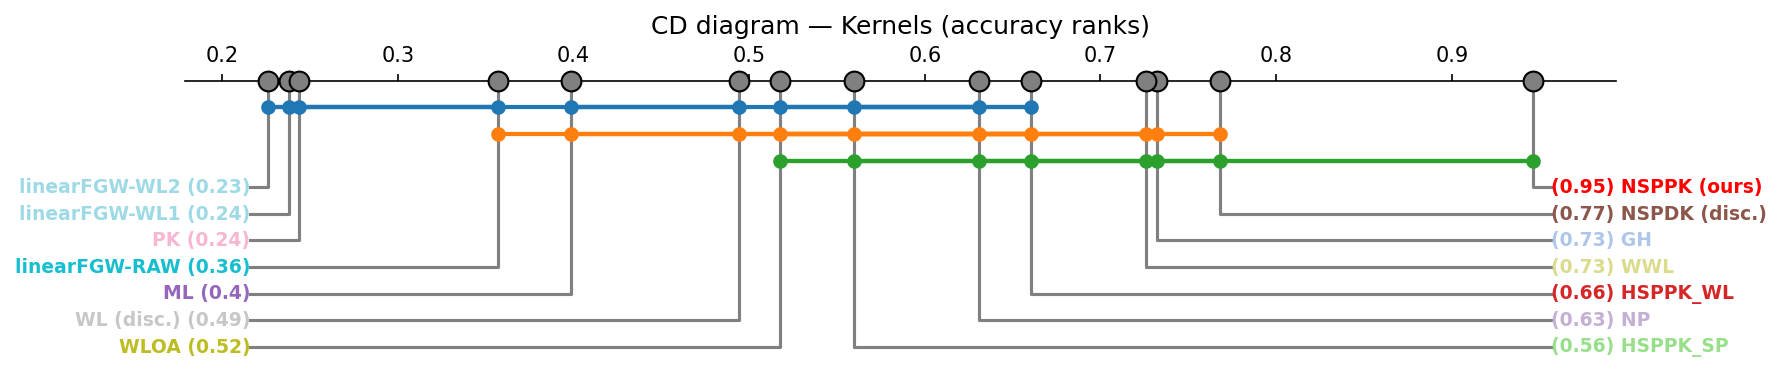
\includegraphics[width=\linewidth]{images/critical_difference_diagram_kernels.png}
\caption{Critical difference diagram for \textbf{kernel} methods on accuracy.
The horizontal axis shows average normalised rank across datasets, scaled to
$[0,1]$ so that higher values indicate better performance. Non-significant
groups under Conover post-hoc testing (Holm-corrected) are indicated by shared
crossbars.}
  \label{fig:cd_kernels}
\end{figure}

\begin{figure}[t]
  \centering
  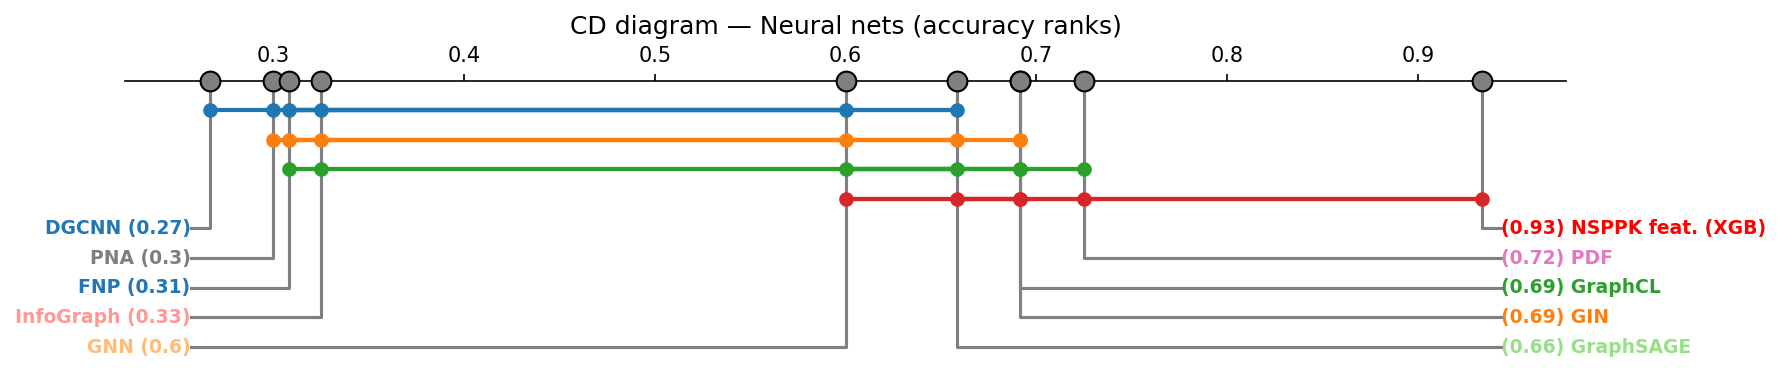
\includegraphics[width=\linewidth]{images/critical_difference_diagram_nn.png}
\caption{Critical difference diagram for \textbf{neural} baselines and the
NSPPK-feature pipeline on accuracy. The horizontal axis shows average normalised
rank across datasets, scaled to $[0,1]$ so that higher values indicate better
performance. Non-significant groups under Conover post-hoc testing
(Holm-corrected) are indicated by shared crossbars.}
  \label{fig:cd_nn}
\end{figure}




\subsection{Parallel Scalability}
\label{sec:parallel}

To evaluate NSPPK's scalability, we vectorized the \textbf{QM9} dataset (\textasciitilde130,000 graphs) using a fixed configuration: \textbf{12-bit hash size}, maximum \textbf{radius = 1}, \textbf{distance = 4}, and \textbf{connector path = 1}. This setup balances expressiveness and efficiency, making it suitable for large-scale benchmarks. As shown in Figure~\ref{fig:appendix_scaling_plot}, the total vectorisation time decreases almost linearly with the number of CPU cores, completing in under 10 minutes on 112 cores. This confirms NSPPK's efficient parallelization and practicality for large datasets.

Figure~\ref{fig:appendix_scaling_plot} presents the results on a log-log scale. The x-axis indicates the number of CPU cores, and the y-axis shows the total vectorisation time. The observed trend is close to ideal linear scaling: doubling the number of cores results in approximately half the runtime. This demonstrates that NSPPK's feature extraction process incurs minimal synchronization or coordination overhead.

Experiments were conducted on a dual-socket Intel server equipped with 2× Intel Xeon Gold 6330 CPUs @ 2.00 GHz, each providing 28 physical cores (56 threads), for a total of 112 logical CPU cores. The machine had 2 NUMA nodes, 70 MB of shared L2 cache, and 84 MB of L3 cache.
Despite relying solely on CPU resources, NSPPK scaled efficiently across all available cores. For example, complete vectorisation of the QM9 dataset was achieved in under 10 minutes, demonstrating the method’s practicality for real-world, large-scale deployment.

\begin{figure}[H]
  \centering
  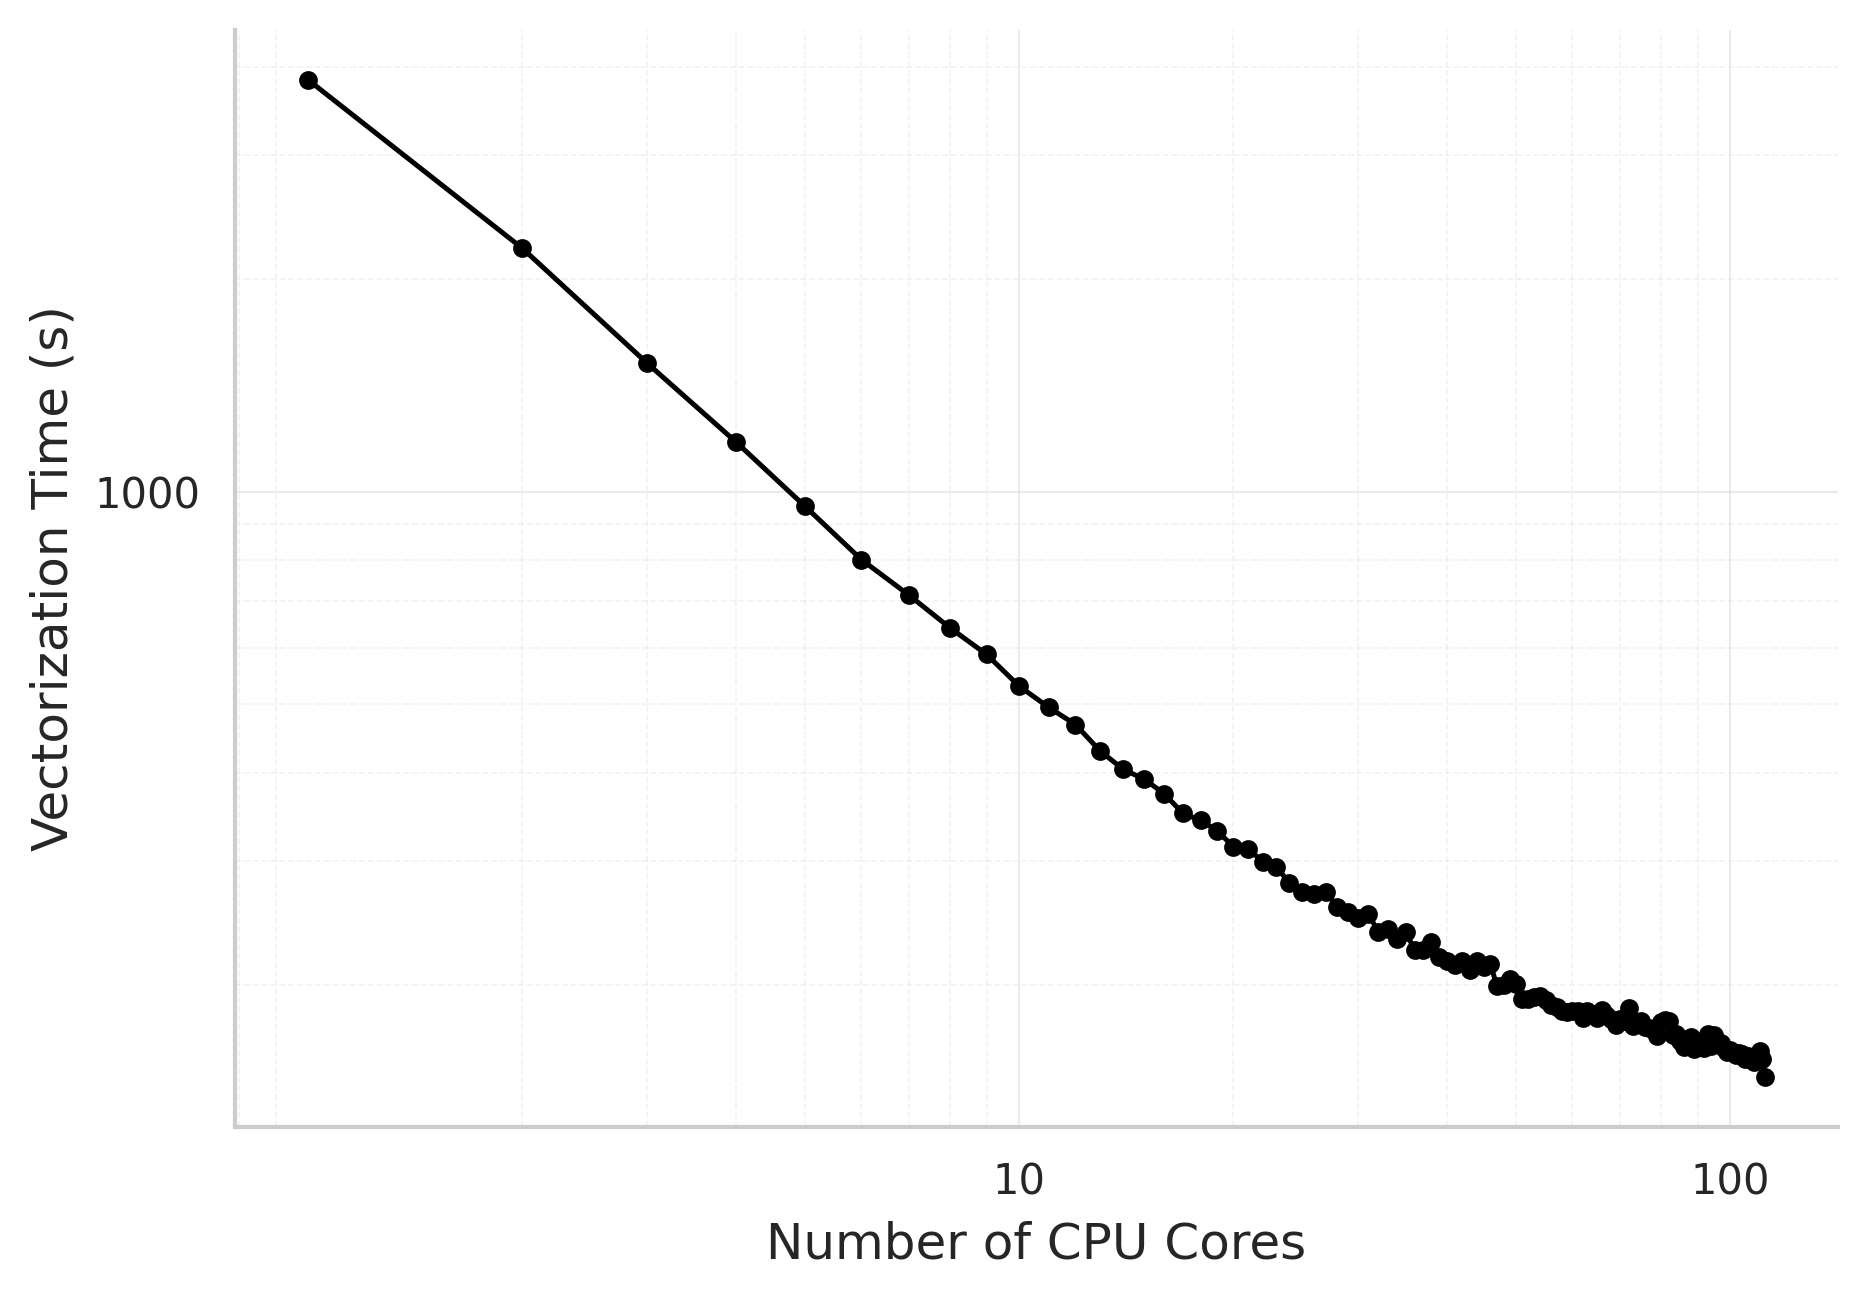
\includegraphics[width=0.5\linewidth]{images/output.png}
  \caption{vectorisation time vs.\ number of CPU cores on QM9 (log-log scale). NSPPK demonstrates excellent parallel scalability, reducing total vectorisation time from over an hour (using a single core) to under 10 minutes with 112 CPU cores. This shows near-linear performance gains with increased parallelization.}
  \label{fig:appendix_scaling_plot}
\end{figure}

\subsection{Ablation Study}
\label{sec:ablation}

We evaluate the contribution of three core components of NSPPK:
(i) distance-based features,
(ii) the union-of-shortest-paths connector, and
(iii) the high-degree thresholding heuristic.
All experiments use a fixed configuration ($R=1$, $D=4$, $r'=1$) with a
\texttt{RandomForestClassifier}.
Table~\ref{tab:ablation} reports classification accuracy across datasets.
While the impact of individual components varies by dataset, the full NSPPK
model consistently matches or outperforms all ablated variants.
In particular, degree thresholding yields a robust improvement across datasets,
supporting its role in mitigating high-degree neighbourhood specificity.
The behavior of NSPPK under increasing graph density, including the effects of
degree thresholding and connector features, is analyzed in
Appendix~\ref{appendix:density_sensitivity}.
\begin{table}[H]
\centering
\caption{Ablation study: Accuracy (\%) $\pm$ Std.}
\label{tab:ablation}
\scriptsize
\setlength{\tabcolsep}{3pt}
\begin{adjustbox}{max width=\columnwidth}
\begin{tabular}{lcccccc}
\toprule
\textbf{Setting} & \textbf{ENZYMES} & \textbf{BZR} & \textbf{PROTEINS} & \textbf{DHFR} & \textbf{SYNTHETICnew} & \textbf{COX2} \\
\midrule
No Distance        & 57.17 $\pm$ 6.99 & 85.69 $\pm$ 5.52 & 76.37 $\pm$ 3.85 & 80.17 $\pm$ 4.35 & 98.33 $\pm$ 2.24 & 81.16 $\pm$ 2.45 \\
No Path            & 52.83 $\pm$ 6.28 & 86.98 $\pm$ 3.72 & 76.10 $\pm$ 4.11 & 76.85 $\pm$  2.58 & 98.67 $\pm$ 1.63 & 80.73 $\pm$ 2.30 \\
No Threshold       & 55.50 $\pm$ 4.48 & 87.42 $\pm$ 2.25 & 75.92 $\pm$ 5.05 & 83.34 $\pm$ 3.10 & 99.00 $\pm$ 1.53 & 81.81 $\pm$ 3.78 \\
\textbf{Full NSPPK}& \textbf{57.83 $\pm$ 5.43} & \textbf{87.90 $\pm$ 3.56} & \textbf{76.20 $\pm$ 3.74} & \textbf{82.95 $\pm$ 4.57} & \textbf{99.00 $\pm$ 1.53} & \textbf{82.46 $\pm$ 3.74} \\
\bottomrule
\end{tabular}
\end{adjustbox}
\end{table}
\subsubsection{Hyperparameter Sensitivity Analysis}
\label{sensitivity}


We study how predictive performance varies with the anchor radius $R$, distance
parameter $D$, and connector radius $R'$. On the COX2 dataset, we perform a
stratified 10-fold cross-validation experiment, varying one parameter at a time
while keeping the other two fixed at $(R,D,R')=(1,4,1)$. Table~\ref{tab:sensitivity}
reports mean classification accuracy and standard deviation across folds, with
values shown as fractions.

Across all three sweeps, performance remains stable: mean accuracy stays in the
range $0.79$--$0.81$ across the tested settings. This variation is small relative
to the fold-level standard deviations, suggesting that NSPPK is not highly
sensitive to fine-grained tuning of $(R,D,R')$ on this dataset. This behaviour is
consistent with small, sparse molecular graphs, where larger radii tend to add
redundant or quasi-global patterns rather than genuinely new local substructures.
\begin{table}[H]
\centering
\caption{Sensitivity of NSPPK accuracy to structural parameters on COX2
(stratified 10-fold cross-validation). Entries report mean accuracy $\pm$
standard deviation across folds, shown as fractions. Each column varies one
hyperparameter while fixing the others at $(R,D,R')=(1,4,1)$.}
\label{tab:sensitivity}
\label{tab:coxsensitivity}
\scriptsize
\setlength{\tabcolsep}{4pt}
\begin{tabular}{cccc}
\toprule
Value & Radius $R$ & Distance $D$ & Connector $r'$ \\
\midrule
0 & $0.81 \pm 0.05$ & $0.81 \pm 0.05$ & $0.81 \pm 0.05$ \\
1 & $0.81 \pm 0.05$ & $0.81 \pm 0.05$ & $0.81 \pm 0.05$ \\
2 & $0.80 \pm 0.03$ & $0.80 \pm 0.04$ & $0.79 \pm 0.03$ \\
3 & $0.80 \pm 0.05$ & $0.80 \pm 0.05$ & $0.80 \pm 0.03$ \\
4 & $0.80 \pm 0.03$ & $0.81 \pm 0.05$ & $0.80 \pm 0.04$ \\
5 & $0.80 \pm 0.03$ & $0.80 \pm 0.04$ & $0.79 \pm 0.04$ \\
6 & $0.79 \pm 0.03$ & $0.80 \pm 0.04$ & $0.80 \pm 0.04$ \\
\bottomrule
\end{tabular}
\end{table}
\subsubsection{Density-Sensitivity Experiment}
\label{appendix:density_sensitivity}

To explicitly study the impact of graph density on runtime, we conducted a
controlled \emph{density-sensitivity experiment} on synthetic Erdős--Rényi
graphs. This experiment complements our theoretical complexity analysis by
measuring how-
NSPPK feature extraction scales as the average node degree
increases.
We generated graphs according to the Erdős--Rényi model $G(n,p)$ with a fixed
number of nodes $n = 300$ and varying expected average degree $k$.
For each value of $k$, the edge probability was set to
$p = k/(n-1)$.
All graphs were assigned trivial, identical labels and no node attributes so as
to isolate the effect of graph density.
We measured the  time required to extract NSPPK features using our
standard configuration $(R=1, D=4, R'=1, nbits=11)$
For each $k$, a single graph instance was generated and timed.
Table~\ref{tab:density_sensitivity} reports NSPPK feature extraction time as a
function of the average degree.
\begin{table}[h]
\centering
\caption{NSPPK feature extraction time vs.\ average graph degree on
Erdős--Rényi graphs ($n=300$).}
\label{tab:density_sensitivity}
\scriptsize
\setlength{\tabcolsep}{6pt}
\begin{tabular}{cc}
\toprule
\textbf{Avg.\ Degree} & \textbf{Time (s)} \\
\midrule
2   & 2.29   \\
27  & 66.11  \\
52  & 102.40 \\
77  & 150.75 \\
102 & 202.39 \\
127 & 256.25 \\
152 & 308.38 \\
177 & 355.59 \\
202 & 388.98 \\
227 & 412.80 \\
252 & 425.54 \\
277 & 429.48 \\
\bottomrule
\end{tabular}
\end{table}
\paragraph{Discussion.}
As the average degree increases from $2$ to $277$, the feature extraction time
grows  from approximately $2.3\,\mathrm{s}$ to $430\,\mathrm{s}$.
The observed runtime trend is close to linear in $|E|$ for fixed graph size, consistent with the bounded-radius BFS analysis in Appendix~\ref{appendix:complexity}, while higher-degree regimes approach the quadratic worst case.
Notably, even in the near-complete regime (average degree $\approx 277$ out of a
maximum of $299$), NSPPK remains computationally practical, requiring only a few
minutes to process a dense $300$-node graph.

\subsection{Experiments on Citation Networks}
\label{sec:citation}

To evaluate whether NSPPK generalises beyond molecular graphs,
we conducted additional experiments on three widely used citation
network benchmarks: \textbf{Cora}, \textbf{CiteSeer}, and \textbf{PubMed}.
These graphs differ substantially from molecular datasets, exhibiting
higher-degree outliers, broader graph diameters, and citation-style
connectivity patterns.

We compared NSPPK against several common graph neural network
architectures for node classification, including
GCN~\citep{kipf2017semi}, GAT
~\citep{velivckovic2018gat},
GraphSAGE~\citep{hamilton2017graphsage}, GIN~\citep{xu2019powerful},
SGC~\citep{wu2019simplifying}, and APPNP~\citep{klicpera2019predict},
as well as a feature-only MLP baseline.

All models were evaluated using an 80/20 train--test split.
Table~\ref{tab:citation_results} reports macro-averaged ROC--AUC scores.

\begin{table*}[t]
\centering
\caption{Test ROC--AUC (macro, one-vs-rest) on citation networks.}
\label{tab:citation_results}
\setlength{\tabcolsep}{4pt}

\begin{adjustbox}{max width=\textwidth}
\begin{tabular}{lcccccccc}
\toprule
Dataset
& GraphSAGE
& GAT
& APPNP
& GCN
& SGC
& NSPPK+XGB
& MLP
& GIN \\
\midrule
CiteSeer
& 0.9422 & 0.9454 & 0.9310 & 0.9257 & 0.9432 & 0.9253 & 0.9247 & 0.9084 \\
Cora
& 0.9846 & 0.9874 & 0.9884 & 0.9840 & 0.9874 & 0.9636 & 0.9502 & 0.9669 \\
PubMed
& 0.9759 & 0.9615 & 0.9622 & 0.9659 & 0.9396 & 0.9686 & 0.9714 & 0.9663 \\
\bottomrule
\end{tabular}
\end{adjustbox}
\end{table*}

Despite using the same hyperparameters as in the molecular experiments,
NSPPK achieves competitive performance across all citation datasets.
These results show that NSPPK generalises well to non-molecular
domains and heterogeneous graph topologies while maintaining predictable
runtime and deterministic feature extraction.

Implementation details and preprocessing steps for the citation network
experiments are provided in Appendix~\ref{appendix:citation}.
\subsection{Structural-only setting.}
To isolate the structural contribution of the representations, we also
evaluated all methods after removing node attributes. The resulting
classification accuracy and runtime comparisons are reported in
Appendix~\ref{appendix:no_attr} and
Appendix~\ref{appendix:no_attr_runtime}. NSPPK maintains competitive
performance in this setting, indicating that its representation captures
meaningful structural information even without attribute features.
\subsection{Large-Scale Evaluation}
\label{sec:large}

We evaluate NSPPK on the large-scale \texttt{ogbg-molpcba} benchmark from the
Open Graph Benchmark~\citep{hu2020ogb}, which contains 437,929 molecular graphs
with node attributes and 128 binary classification tasks. Each baseline was
trained once on the official OGB scaffold split (249,715 train, 29,826
validation, 29,427 test). Using a fixed configuration
($R=1$, $D=4$, $R'=1$, $b=16$, we computed explicit NSPPK
features for the entire dataset in under one hour on CPU.

Across all tasks, NSPPK achieves an average validation AP of 0.22 and test AP
of 0.21 without hyperparameter tuning, pretraining, or GPU acceleration.
In contrast, state-of-the-art neural models such as
Graphormer~\citep{ying2021transformers},
PDF~\citep{yang2023pdf}, and
HyperFusion~\citep{ye2025hyperfusion}
typically achieve test AP values of 0.30--0.32, while tuned mid-range models
such as PNA~\citep{corso2020pna} and GIN~\citep{xu2019powerful} reach
approximately 0.25--0.30.

To further analyze sample efficiency, we conducted a focused study on
\textbf{task~95} of \texttt{ogbg-molpcba}, which contains 48,853 positive
examples and 293,968 negative examples. Balanced subsets of increasing size
were constructed to evaluate performance as a function of training data
availability.

Figure~\ref{fig:large_experiment} shows the resulting learning curves.
NSPPK demonstrates strong sample efficiency, outperforming neural baselines at
small training sizes while maintaining substantially lower computational cost,
particularly in its sparse representation. At larger training sizes,
neural architectures such as PDF eventually surpass NSPPK in predictive
performance, although the gap remains modest.

Implementation details for the task~95 experiments, including classifier
configurations and neural baseline settings, are provided in
Appendix~\ref{appendix:task95}.

\begin{figure*}[ht]
  \centering
  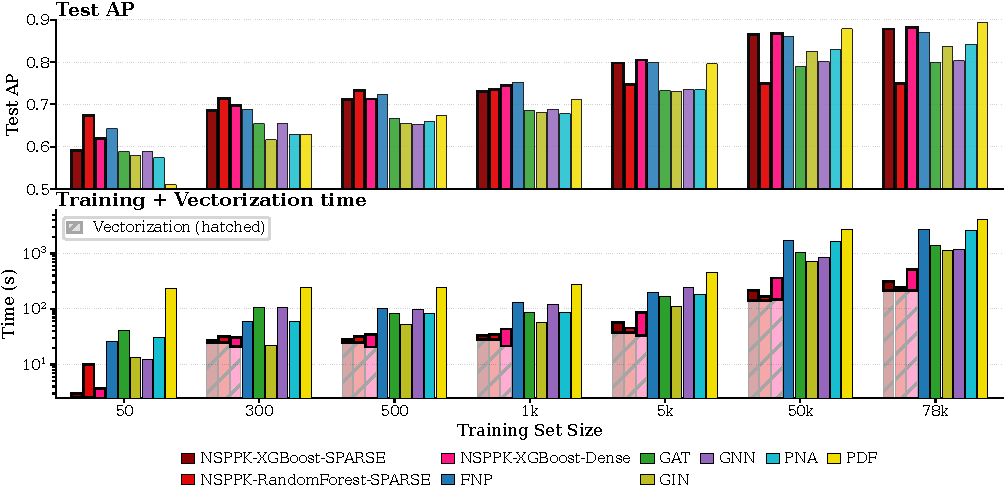
\includegraphics[width=.95\textwidth]{images/icml_compact_learning_curves.pdf}
  \caption{Learning curves on \texttt{ogbg-molpcba} (task~95).
  NSPPK (red) compared with neural baselines including GIN, GAT, PNA,
  PDF, and AttentiveFP (FNP).}
  \label{fig:large_experiment}
\end{figure*}
\section{Discussion and Limitations}
\label{sec:nsppk:discussion-limitations}

The results show that NSPPK can provide competitive graph-level features while
remaining deterministic and explicit. Its main advantage is that each active
dimension is tied to a hashed structural pattern involving anchor
neighbourhoods, connector paths, and attribute information. This supports
feature inspection: important coordinates can be traced back to the kinds of
substructures that produced them. The interpretation is therefore local to the
constructed feature map and the downstream model coefficients; it should not
be read as a complete causal explanation of a prediction.

The method also has practical limits. Feature extraction depends on the chosen
radii, anchor distances, and hash size. Larger values can capture richer
structure, but they also increase runtime and sparsity, especially on dense
graphs. Hashing makes the representation compact and efficient, but distinct
patterns may collide when the hash space is too small. The robustness analysis
therefore complements the classification results by testing whether the kernel
continues to produce meaningful similarities under controlled perturbations,
rather than assuming that sparsity alone is harmless.

Finally, NSPPK is a predefined representation. It does not learn which
substructures are useful before feature extraction; this choice is made by the
kernel design and its parameters. This can improve sample efficiency and
auditability, but it also means that task-specific adaptation is left to the
downstream learner. Hybrid approaches that use NSPPK features as inputs,
regularisers, or conditioning descriptors for neural graph models remain a
natural direction for future work.

\section{Conclusion}
\label{sec:Conclusion}

We introduced NSPPK, an explicit graph kernel that extends classical
neighbourhood-based representations through connector substructures and direct
integration of continuous node attributes, yielding sparse and interpretable
graph-level embeddings.  NSPPK belongs to the class of predefined,
data-independent methods while enriching their expressive power through richer
structural encoding.

NSPPK provides deterministic and training-free feature extraction, enabling
scalable graph learning with standard supervised models. Empirically, it
achieves the best average rank among the tested graph kernels and competitive
results against the neural baselines considered in this chapter, despite
avoiding representation learning or end-to-end optimisation. These results show
that carefully designed explicit representations can remain useful alongside
learned embeddings. Because NSPPK features correspond to hashed subgraph
patterns, predictive signals can be inspected by retrieving the structural
patterns associated with important feature coordinates.

Within the broader perspective of this thesis, NSPPK advances the
\emph{representation} component of graph learning. The next chapter complements
this direction by studying \emph{generation}, focusing on diffusion-based graph
models that learn probabilistic representations of graph distributions. While
NSPPK emphasises explicit structural encoding, diffusion models prioritise
flexible data-driven synthesis, together forming complementary approaches to
graph learning.

Future work includes hybrid kernel–neural models and extensions to dynamic or
temporal graphs.
